%% Bookheader, Nov 8, 2020; July 18, 2022

\documentclass[11pt]{../Support/ourbook}
%% or for landscape, comment out line above and use this one:
%%\documentclass[landscape,11pt]{ourbook}

%% This will keep space from stretching around display math:

\makeatletter
\renewcommand\normalsize{%
   \@setfontsize\normalsize\@xipt{13.6}%
   \abovedisplayskip 11\p@  \@minus6\p@
   \abovedisplayshortskip \z@ 
   \belowdisplayshortskip 6.5\p@ \@minus3\p@
   \belowdisplayskip \abovedisplayskip
   \let\@listi\@listI}
\makeatother
\normalsize


\begin{document}

\tableofcontents
\graphicspath{{../../Chapters/emwaves/en_US}}
\chapter{Electromagnetic Waves}

Sound is a compression wave -- to travel, it needs a medium to
compress: air, water, etc. (Regardless of what you have seen in
movies, sound does not travel through a vacuum)

Light is an electromagnetic wave -- it causes fluctuations in the
electric and magnetic fields that are everywhere. It can cross a
vacuum, as it does to reach us from the sun.

Electromagnetic waves travel at about 300 million meters per second in a
vacuum. The waves travel slower through things. For example, an
electromagnetic wave travels at 225 million meters in water.

Electromagnetic waves come in different frequencies. For example, the
light coming out of a red laser pointer is usually about $4.75 \times
10^{14}$ Hz.  The wifi data sent by your computer is carried on an
electromagnetic wave too. It is usually close to $2.4 \times 10^6$ Hz
or $5 \times 10^6$ Hz.

Because we know how fast the waves are moving, we sometimes talk about
their wavelengths instead of their frequencies.  The light coming out
of a laser pointer is $300 \times 10^6 / 4.76 \times 10^{14} = 630
\times 10^{-9}$ m, or 630 nm.

\begin{Exercise}[title={Wavelengths}, label=wave_length_green]

  A green laser pointer emits light at $5.66 \times
10^{14}$ Hz. What is its wavelength in a vacuum?
  
\end{Exercise}
\begin{Answer}[ref=wave_length_green]
$$\frac{300 \times 10^6}{5.66 \times 10^{14}} = 530 \times 10^{-9} = 530\text{ nm}$$
\end{Answer}

We have given names to different ranges of the electromagnetic spectrum:

\begin{tabular}{r | l | l}
  Name & Hertz & Meters \\
  \hline
Gamma rays  & $  \times 10^{}$ &$ \times 10^{}$\\
X-rays  & $ \times 10^{}$&$ \times 10^{}$\\
Ultraviolet  & $ \times 10^{}$&$ \times 10^{}$\\
Blue & $ \times 10^{}$&$ \times 10^{}$\\
Red  & $ \times 10^{}$&$ \times 10^{}$\\
Infrared  & $ \times 10^{}$&$ \times 10^{}$\\
Microwaves  & $ \times 10^{}$&$ \times 10^{}$\\
Radio waves  & $ \times 10^{}$&$ \times 10^{}$\\
\end{tabular}

(You may have heard of ``cosmic rays'' and wonder why they are
not listed in this table. Cosmic rays are actually the nuclei of atoms
that have been stripped of their electron cloud. These particles come
flying out of the sun at very high speeds. They were originally
thought to be electromagnetic waves, and they were mistakenly named
``rays''.)

In general, the lower frequency the wave is, the better it passes
through a mass.  A radio wave, for example, can pass through the walls
of your house, but visible light cannot.  The people who designed the
microwave oven, chose the frequency of 2.45 GHz because the energy
from those waves tended to get absorbed in the first few inches of
food that it passed through.

\section{The greenhouse effect}

Humans have dug up a bunch of long carbon-based molecules (like oil
and coal) and burned them, releasing large amounts of $CO_2$ into the
atmosphere. It is not obvious why that has made the planet warmer. The
answer is electromagnetic waves.

A warm object gives off infrared electromagnetic waves. That's why,
for example, motion detectors in security systems are actually
infrared detectors: even in a dark room, your body gives off a lot of
infrared radiation.

You may have heard of ``heat-seeking missiles.'' These are more
accurately called ``Infrared homing missiles'' because they follow
objects giving off infrared radiation -- hot things like jet engines.

The sun beams a lot of energy to our planet in the form of
electromagnetic radiation: visible light, infrared, ultraviolet. (How
much? At the top of the atmosphere directly facing the sun, we get
1,360 watts of radiation per square meter. That is a lot of power!)

Some of that radiation just reflects back into space.  23\% is
reflected by the clouds and the atmosphere, 7\% makes it all the way
to the surface of the planet and is reflected back into space.

The other 71\% is absorbed: 48\% is absorbed by the surface and 23\%
is absorbed by the atmosphere. All of that energy warms the planet and
the atmosphere so that it gives off infrared radiation. The planet
lives in equilibrium: The infrared radiation leaving our atmosphere is
exactly the same amount of energy as that 71\% of the radiation that
it absorbs.

(If the planet absorbs more energy than it releases, the planet gets
hotter.  Hotter things release more infrared. When the planet is in
equilibrium again, it stops getting hotter.)

So what is the problem with $CO_2$ and other large molecules in the
atmosphere? They absorb the infrared radiation instead of letting it
escape into space. Thus the planet must be hotter to maintain
equilibrium.
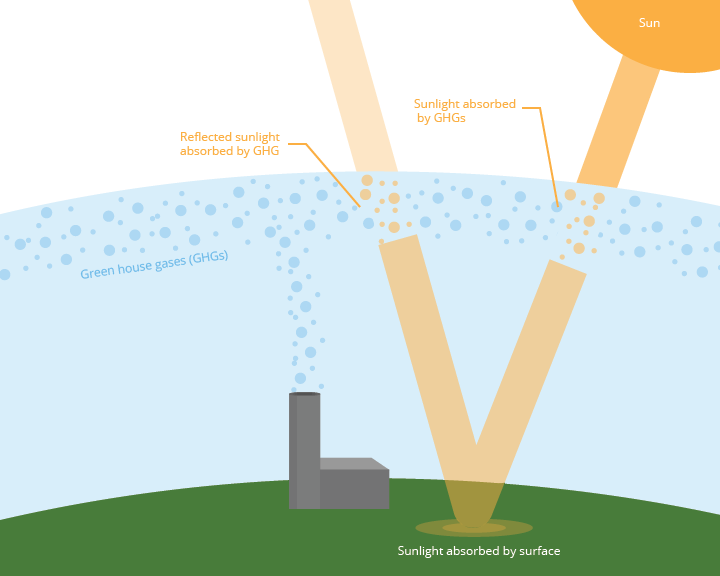
\includegraphics[width=1\textwidth]{ghgEffect.png}

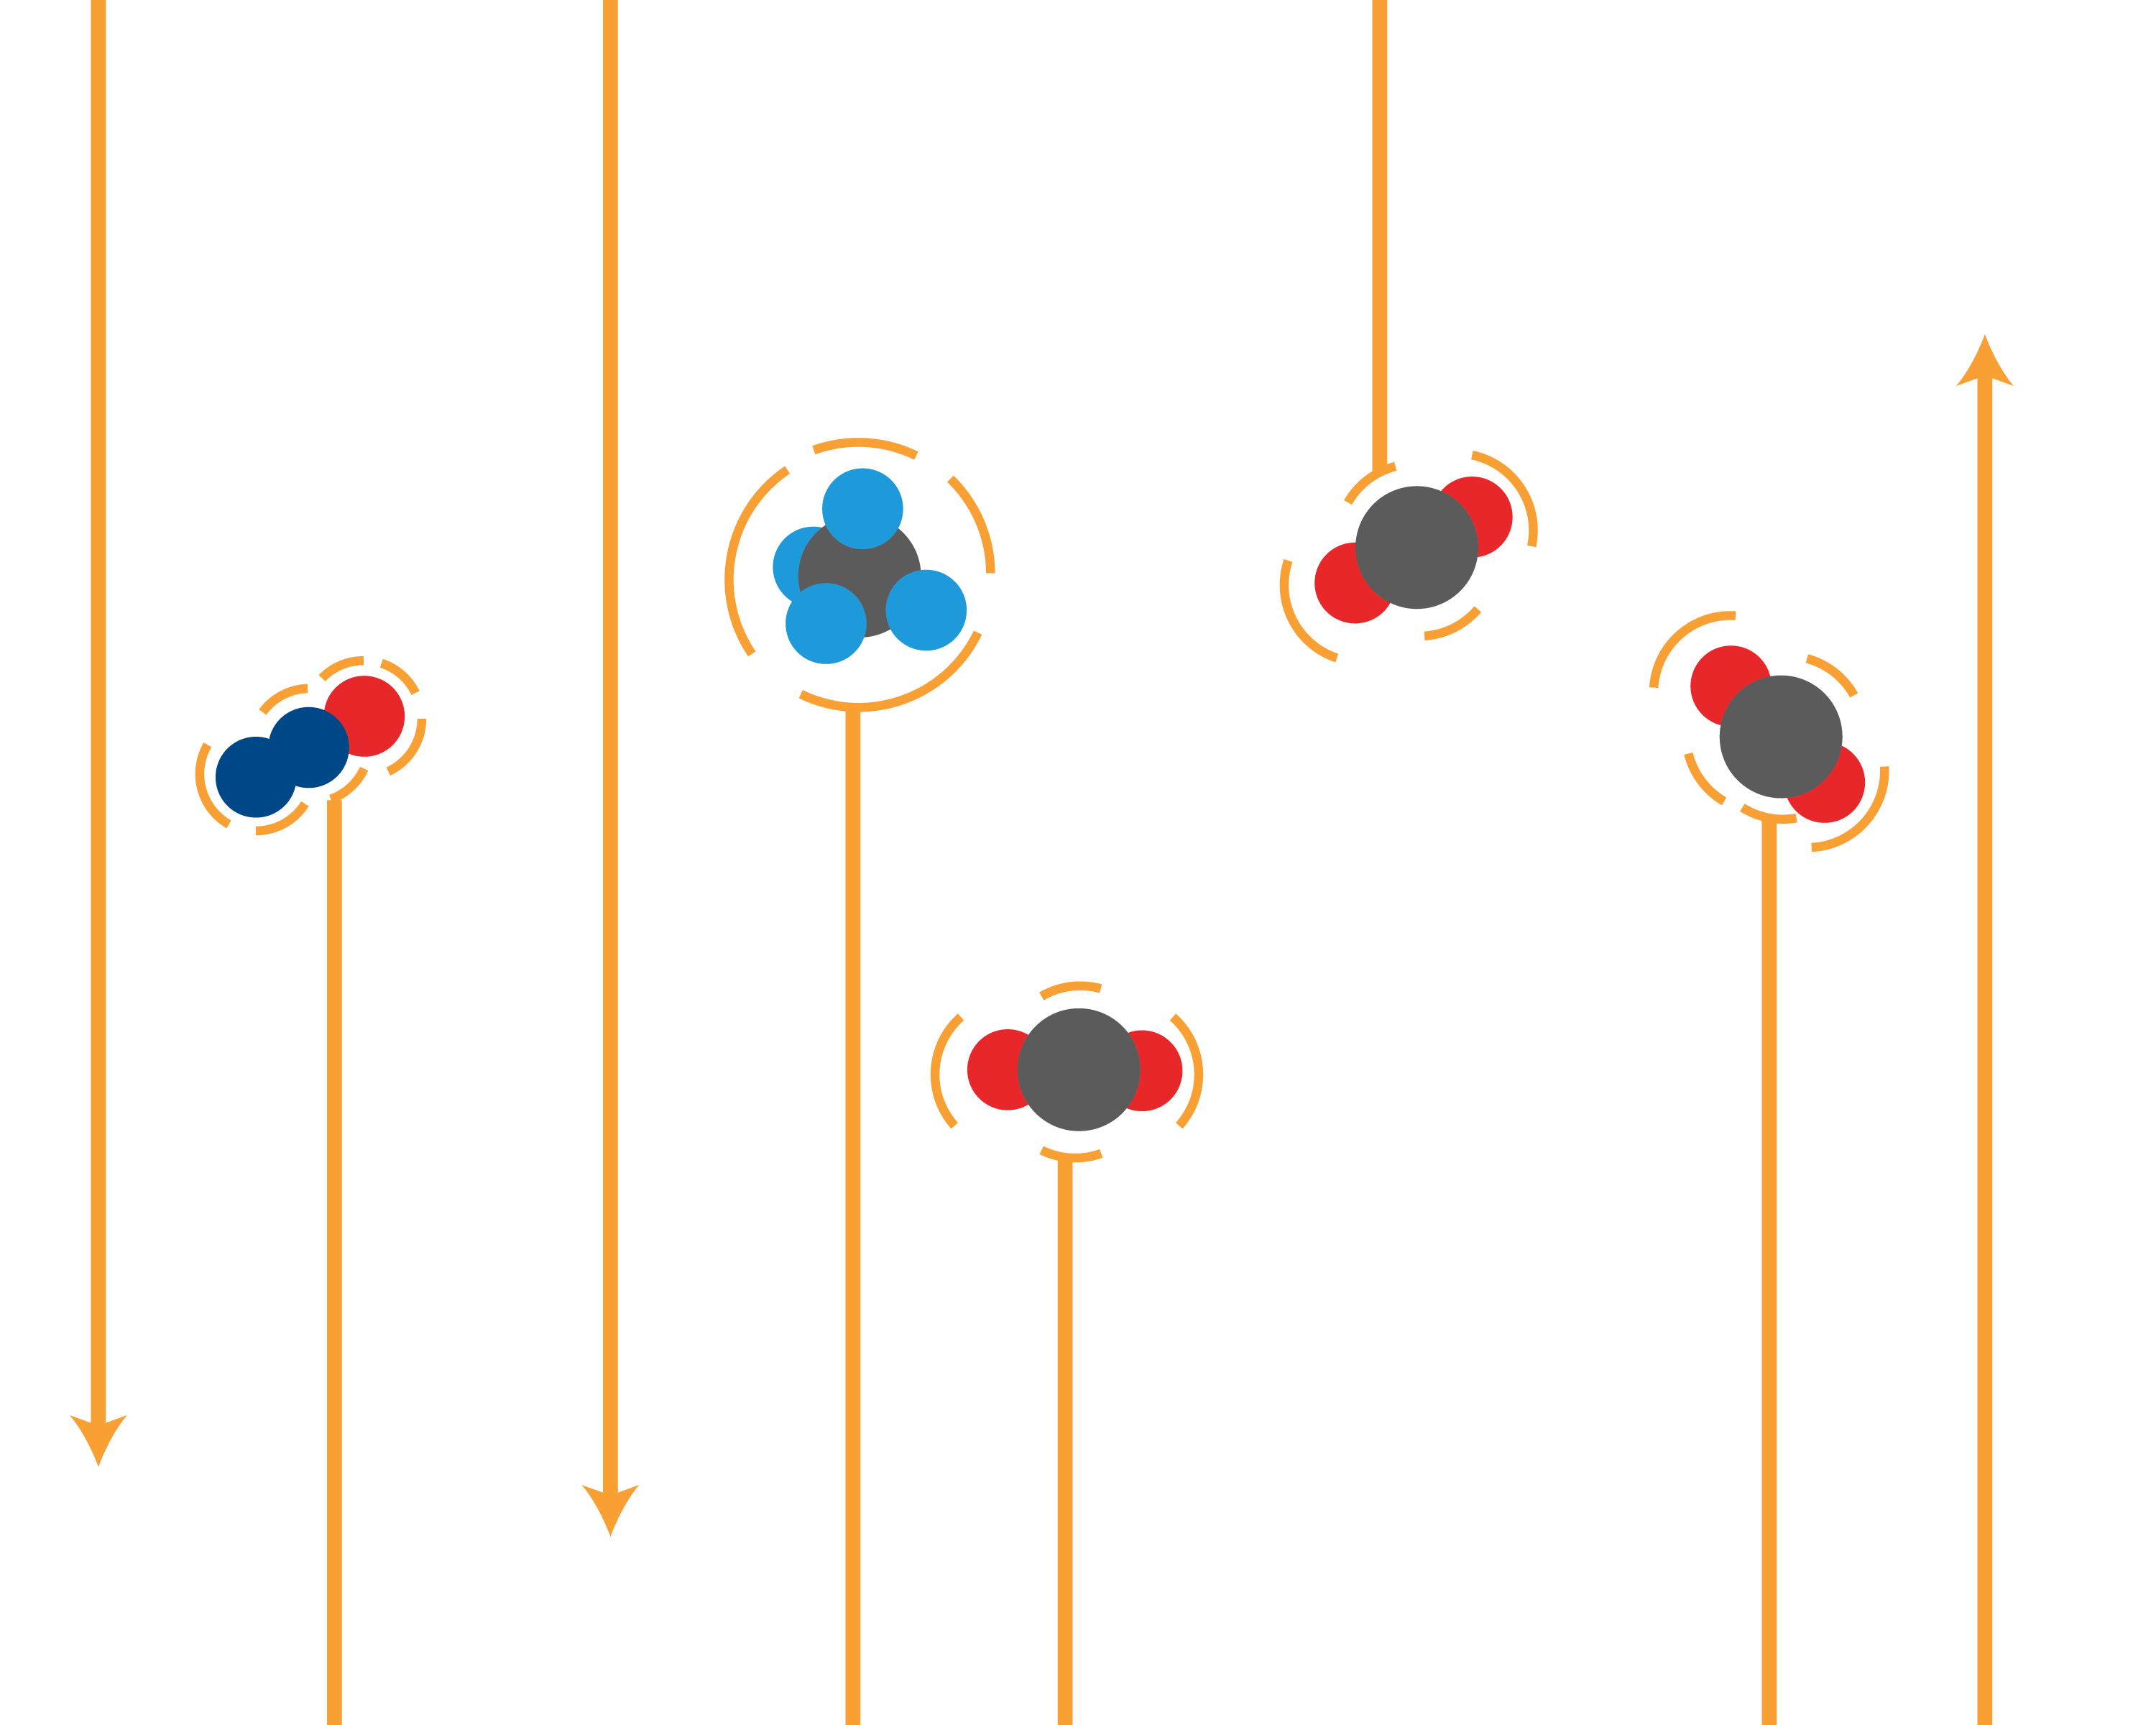
\includegraphics[width=1\textwidth]{ghgClose.png}

The planet is getting hotter, and it is creating a multitude of
problems:
\begin{itemize}
\item Weather patterns are changing, which leads to extreme floods and
  droughts.
  
\item Ice and snow in places like Greenland are melting and flowing
  into the oceans. This is raising sea-levels.
  
\item Biomes with biodiversity are resilient. Rapidly changing climate
  is destroying biodiversity everywhere, which is making these ecosystems
  very fragile.
  
\item In many places, permafrost, which has trapped large amounts of
  methane in the ground for millenia, is melting.
\end{itemize}

That last item is particularly scary because methane is a large gas
molecule -- it absorbs even more infrared radiation than $CO_2$. As it is
escapes the permafrost, the problem will get worse.

Scientists are working on four kinds of solutions:
\begin{itemize}
  \item \textbf{Stop increasing the amount of greenhouse gases in our
    atmosphere.} It is hoped that non-carbon based energy systems like
    solar, wind, hydroelectric, and nuclear could let us stop burning
    carbon. Given the methane already being released, it maybe too
    late for this solution to work on its own.

  \item \textbf{Take some of greenhouse gases out of our atmosphere and
    sequester them somewhere.} The trunk of a tree is largely carbon
    molecules. When you grow a tree where there had not been one
    before, you are sequestering carbon inside the tree.  There are
    also scientists that are trying to develop process that pull
    greenhouse gases out of the air and turn them into solids.

  \item \textbf{Decrease the amount of solar radiation that is
    absorbed by our planet and its atmosphere.} Clouds reflect a lot of radiation back into
    space. Could we increase the cloudiness of our atmosphere? Or
    maybe  mirrors in orbit around our planet?

  \item \textbf{Adapt to the changing climate.} These scientists are
    assuming that global warming will continue, and are working to
    minimize future human suffering. How will we relocate a billion
    people as the oceans claim their homes?  When massive heat waves
    occur, how will we keep people from dying?  As biodiversity
    decreases, how can we make sure that species that are important to
    human existence survive?
    
\end{itemize}

What are the greenhouse gases and how much does each contribute to
keeping the heat from exiting to space?  These numbers are still being
debated, but this will give you a feel:
\begin{tabular}{c | c | c}
  Water vapor & $H_2O$ & 36 - 72 \% \\
  Carbon dioxide & $CO_2$ & 9 - 26 \% \\
  Methane & $CH_4$ & 4 - 9 \% \\
  Ozone & $O_3$ & 3 - 7 \%
\end{tabular}

Notice that while we talk a lot about carbon dioxide, the most
important greenhouse gas is actually water.  Why don't we talk about
it? Given the enormous surfaces of the oceans, it is difficult to
imagine any way to permanently decrease the amount of water in the
air. Also, a lot of water in the air is in the form of clouds that
help reflect radiation before it is absorbed.


\graphicspath{{../../Chapters/camera/en_US}}
\chapter{How Cameras Work}

Let's say it is a sunny day and you are standing in field a few meters
from a cow. You use the camera on your phone to take a picture of the
cow. How does that whole process work?

\section{The Light That Shines On the Cow}

The sun is a sphere of hot gas. About 70\% of the gas is
hydrogen. About 28\% is helium. There's also a little carbon, nitroge,
and oxygen.

Gradually, the sun is converting hydrogen into helium through a
process known as ``nuclear fusion''. (We will talk more about nuclear
fusion in a later chapter.) A lot of heat is created in this
process. The heat makes the gases glow.

How does heat make things glow? The heat pushes the electrons into
higher orbitals.  When the fall back down to a lower orbital, they
release a photon of energy, which travels away from the atam as an
electromagnetic wave.

Heat isn't the only way to push the electrons into a higher
orbital. For example, a flourescent lightbulb is filled with gas.
When we pass electricity through the gas, its electrons are moved to a
higher orbital.  When they fall, light is created.

What is the frequency of the wave that the photon travels on?
Depending on what orbital it falls from and how far it falls, the
photon created has different amounts of energy. The amount of energy
determines the frequency of the electromagnetic wave.

\begin{mdframed}[style=important, frametitle={Formula for enegy of a photon}]

If you want to know the amount of energy $E$ in a photon, here is the formula:

$$E = \frac{h c}{\lambda}$$

where $c$ is the speed of light, $\lambda$ is the wavelength of the
electromagnetic wave, and $h$ Planck's constant: $6.63 \times 10^{-34} m^2 kg/s$

For example, a red laser light has a wavelength of about 630 nm. So the energy in each photon is:

$$\frac{(300 \times 10^6) (6.63 \times 10^{-34})}{630 \times 10^{-9}} = 3.1 \times 10^{-19} \text{ joules}$$

\end{mdframed}

In the sun, there are several kinds of molecules and each has a few
different orbitals that the electrons can live in.  Thus, the light
coming from the sun is made up of electromagnetic waves of many
different frequencies.

We can see some of these frequencies as different colors, but some are
invisible to humans, for example ultraviolet and infrared.

\section{Light Hits the Cow}

When these photons from the sun hit the cow, the hide and hairs of the
cow will absorb some of the photons. These photons will become heat
and make the cow feel warm.  Some of the photons will not be absorbed
-- they will leave the cow.  When you say ``I see the cow,'' what you are
really saying is ``I see some photons that were not absorbed by the cow.''

Different materials absorb different amounts of each wavelength. A
plant, for example, absorbs large percentage of all blue and red
photons that hit it, but it absorbs only a small percentage of the
green photons that hit it.  Thus we say ``That plant is green.''

White things absorb very small percentages of photons of any visible
wavelength.  Black things absorb very \emph{large} percentages of
photons of any visible wavelength.

Before we go on, let's review: The sun creates photons that travel as
electromagnetic waves of assorted wavelengths to the cow.  Many of
those photons are absorbed, but some are not.  Some of those photons
that are not absorbed go into the lens of our camera.

\section{Pinhole camera}

The simplest cameras have no lenses. They are just a box.  The box has
a tiny hole that allows photons to enter.  The side of the box
opposite the hole is flat and covered with film or some other
photo-sensitive material.

The photons entering the box continue in the same direction they were
going when they passed through the hole.  Thus, the photons that
entered from high, hit the back wall low.  The photons that came from
the left, hit the back wall on the right. Thus the image is projected
onto the back wall rotated 180 degrees: What was up is down, what was
on the left is on the right.

FIXME: picture here

\begin{Exercise}[title={Height of the image}, label=image_height]

Let's say that that the pinhole is exactly the same height as the
shoulder of the cow and that the shoulder is directly above one hoof.
Than the pinhole, the shoulder, and the hoof form a right triangle.

Now, let's say that the camera is being held perpendicular to the
ground.  Now, the pinhole, the image of the shoulder, and the image of
the hoof on the back wall of the camera also form a right triangle.

These two triangles are similar.

The shoulder is 2 meters from the hoof.  The cow is standing 3 meters
from the camera.  The distance from the pinhole to the back wall of
the camera is 3 cm.  How tall is the image of the cow on the back wall
of the camera?

\end{Exercise}
\begin{Answer}[ref=image_height]

The two triangles are similar, one is 2 m and 3m.  The other is $x$ cm and 3 cm.

The image of the cow is 2 cm tall.

\end{Answer}

\section{Lenses}

Quick review: A photon leaves the sun in some random direction. It
travels 150 million km from the sun and hits a cow.  It is not
absorbed by the cow, and heads off in a new direction.  It passes
through the pinhole and hits the back wall of the camera.  That seems
incredibly improbable, right?

It actually is kind of improbable, especially if there isn't a lot of
light -- like you are taking the picture at dusk.  To increase the
odds, we added a \newterm{lens} to the camera.

If you focus a lens on a wall, and then you draw a dot on the
wall. The lens is designed such that all the photons from the dot that
hit the lens get redirected to the same spot on the back wall of the
camera -- regardless of which path it took to get to the lens.

FIXME: illustration here

Note that the image still gets flipped.  There is a \newterm{ focal
point } that all the photons pass through.

FIXME: illustration here

The distance from the lens to its focal point is called the lens's
\newterm{focal length}. Telephoto lenses, that let you take big
pictures of things that are far away, have long focal lengths.
Wide-angle lenses have short focal lengths.

\section{Sensors}

The camera on your phone has a sensor on the back wall of the
camera. The sensor is broken up into tiny rectangular regions called
pixels.  When you say a sensor is 6000 by 4000 pixels, we are saying
the sensor is a grid of 24,000,000 pixels: 6000 pixels wide and
4000 pixels tall.

Each pixel has three types of cavities that take in photos. One of the
cavities measures the amount of short wavelength light, like blues and
violets. One of the cavities measures the long wavelength light, like
reds and oranges. One of the cavities measures the intensity of
wavelengths in the middle, like greens.

Thus, if your camera has a resolution of $6000 \times 4000$, the image
is 72,000,000 numbers: Every one of the 24,000,000 pixels yeilds three
numbers: intensity of long wavelength, mid wavelength, and long
wavelength light. We call these numbers ``RGB'' for Red, Green, and
Blue.




\graphicspath{{../../Chapters/eye/en_US}}
\chapter{How Eyes Work}

Dr. Craig Blackwell has made a great video on the mechanics of the
eye. You should watch it: \url{https://youtu.be/Z8asc2SfFHM}

Mechanically, your eye works a lot like a camera.  The eye is a sphere
with two lenses on the front: The outer lens is called the \newterm{cornea}, and the
second lens is just called ``the lens.''

Between the two lenses is an aperture that opens wide when there is
very little light, and closes very small when there is bright light.
The opening is called the \newterm{pupil} and the tissue that forms
the pupil is called the \newterm{iris}. When people talk of the color
of your eyes, they are talking about the color of your iris. The
blackness at the center of your iris is your pupil.

There are two types of photoreceptor cells in your retina: rods and
cones. The rods are more sensitive; in very dark conditions, most of
our vision is provided by the rods. The cones are used when there is
plenty of light, and they let us see colors.

The white part around the outside of the eyeball? That is called the
\newterm{sclera}.

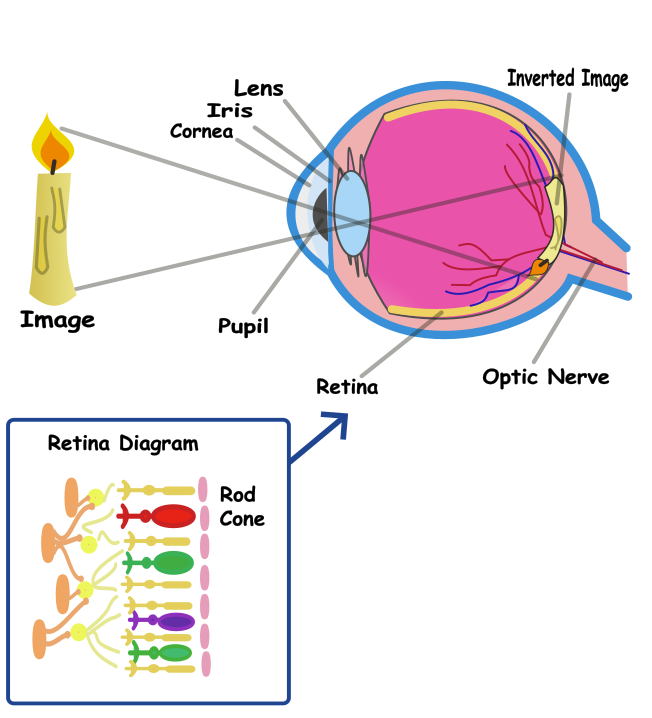
\includegraphics[width=0.8\textwidth]{eye.png}

The walls of the eye are lined inside with the \newterm{retina}, which has
 sensors that pick up the light and send impulses down the optic
nerve to your brain.

Just like a camera, the images are flipped when they get projected on
the back of the eye.

\section{Eye problems}

Now that you know the mechanics of the eye, let's enumerate a few
things that commonly go wrong with the eye.

\subsection{Glaucoma}

The space between your cornea and lens is filled with a fluid called
\newterm{aqueous humor}. To feed the cells of the cornea and lens,
the aqueous humor carries oxygen and nutrients like blood would, but
it is transparent so you can see. Aqueous humor is constantly being
pumped into and out of that chamber.  If aqueous humor has trouble
exiting, the pressure builds up and can damage the eye. This is known
as \newterm{glaucoma}.

\subsection{Cataracts}

The lens should be clear. As a person ages (and it can be accelerated
by diabetes, too much exposure to sunlight, smoking, obesity, and high
blood pressure), the proteins in the lens break down and clump
together, becoming opaque. From the outside, the eye will look
cloudy. This is called a \newterm{cataract}, and it makes it difficult
for the person to see.

The problem can be corrected: The person's cloudy lens is removed and
replaced with a clear, manufactured lens.

\subsection{Nearsightedness, farsightedness, and astigmatism}

If you are in a dark room and a tiny LED is turned on, the photons
from that LED can pass through your cornea in many different places.
If your eye is focusing on that light correctly, all the photons
should meet up at the same place on the retina.

FIXME: Diagram here

If the lenses are bending the light too much, the photons meet up before they hit the
retina and get smeared a bit across the retina. To the person, the LED
would appear blurry. The eye is said to be \newterm{nearsighted} or
\newterm{myopic}.

If the lenses are not bending it enough, the photons would meet up
behind the retina.  Once again, they get smeared a bit across the
retina and the LED looks blurry to the person. The eye is said to be
\newterm{farsighted} or \newterm{hyperoptic}.

Your lenses are supposed to bend the photons the same amount
vertically and horizontally. If one dimension is focused, but the
other is myopic or hyperoptic, the eye is said to have \newterm{astigmatism}.

Myopia, hyperoptia, and astigmatism can be corrected with glasses or contact
lenses. Doctors can also do surgical corrections, usually by changing
the shape of the cornea.

\section{Seeing colors}

TED-Ed has made a good video on how we see color. Watch it here: \url{https://youtu.be/l8_fZPHasdo}

When a rainbow forms, you are seeing different wavelengths separating from each other. In the rainbow:
\begin{itemize}
\item Red is about 650 nm.
\item Orange is about 600 nm.
\item Yellow is about 580 nm.
\item Green is about 550 nm.
\item Cyan is about 500 nm.
\item Blue is about 450 nm.
\item Violet is about 400 nm.
\end{itemize}

If you shine a light with a wavelength of 580 nm on a white piece of
paper, you will see yellow.

However, if you shine two lights with wavelengths of 650 nm (red) and
550 nm (green), you will also see yellow.

Why? Our ears can hear two different frequencies at the same time.
Why can't our eyes see two colors in the same place?

As mentioned above, the cone photoreceptors in our eyes let us see
colors. There are three kinds of cones:
\begin{itemize}
  \item Blue: Cones that are most sensitive to frequencies near 450nm.
  \item Green: Cones that are most sensitive to frequencies near 550nm.
  \item Red: Cones that let us see the frequencies up to about 700nm.
\end{itemize}

When a wavelength of 580 nm hits your retina, it excites the red
and green receptors, and your brain interprets that mix as yellow.

Similarly, when light that contains both 650 nm and 550 nm waves hits
your retina, it excites the red and green receptors, and your brain
interprets that mix as yellow.

You can't tell the difference!

Now we know why the sensors on the camera are RGB. The camera is
recording the scene as closely as necessary to fool your eye.

A TV or a color computer monitor only has three colors of pixels: red,
green, and blue.  By controlling the mix of them, it creates the
sensation of thousands of colors to your eye.

\section{Pigments}

A color printer works oppositely: Instead of radiating
colors, it puts pigments on the paper that absorb certain frequencies.
A pigment that absorbs only frequencies near 650 nm (red) will appear
to your eye as cyan. This makes sense because the sensation of cyan is
created when your blue and green receptors are activated.

Thus, pigment colors come in:
\begin{itemize}
\item Cyan: absorbs frequencies around red
\item Magenta: absorbs freqencies around green
\item Yellow: absorbs frequencies around blue
\end{itemize}

If you buy ink for a color printer, you know there is typically a
fourth ink: black. If you put cyan, magenta, and yellow pigments on
paper, the mix won't absorb all the visible spectrum in a consistent
manner, and our eyes are pretty sensitive to that, so we would see
brown. So we add black ink to get pretty grays and blacks.

We call this approach to color CMYK (as opposed to RGB). If an artist
is creating an image to be viewed on a screen, they will typically
make an RGB image.  If they are creating an image to be printed using
pigments, they typically create a CMYK image. (Most of us don't care
so much -- we just let the computer do conversions between the two
color spaces for us.)


\graphicspath{{../../Chapters/reflection/en_US}}
\chapter{Reflection}

What happens when light hits a mass?

In a previous chapter, we talked about light as a wave, and we
mentioned that each color in the rainbow is a different
wavelength. You can also think of light as particles of energy called
\newterm{photons}. And every photon comes with an amount of energy
that determines what color it is.

When we are talking about light interacting with objects, your
intuition will be right more often if you think of light as a beam of
photons.

When a photon comes from the sun and hits an object, one of several
things can happen:

\begin{itemize}
  
  \item The energy of the photon is absorbed by the object. It makes the
    object a little warmer. If a large proportion of photons hitting the
    mass are absorbed like this, we say the object is ``black''.\index{absorption!photon}

 \item The photon bounces off the object.  If the surface is very
   smooth, the photons bounce in a predictable manner, and we call
   this \newterm{reflection} and we say the object is ``shiny''.\index{reflection}

 \item If the surface is rough and the photons are not absorbed, the
   photons are scattered in random directions.  We call this
   \newterm{diffusion}.  If most of the photons hitting an object are
   bounced in random directions, we say that the object is ``white''.\index{diffusion}

 \item The photon passes through the mass.  If the mass has smooth
   surfaces and a consistent composition, the photons will pass throught the
   mass in a predictable manner.  We say that the mass is ``transparent''.\index{transparent}

 \item If the photons pass through, but in an unpredictable,
   scattering manner, we say the mass is ``translucent''. \index{translucent}

\end{itemize}

No object absorbs every photon, but chemists are always coming up with
``blacker'' materials. Vantablack, for example, is a super-black paint
that absorbs 99.965\% of all photons in the visible spectrum.\index{Vantablack}

No object reflects every photon, but a mirror is pretty close. Let's
talk about reflections in a mirror.\index{mirror}

\section{Reflection}

When a beam of light hits mirror, it bounces of the mirror at the same
angle it approached from.  That is, if it approaches nearly
perpendicular to the mirror, it departs nearly perpendicular to the
mirror.  If it hits the mirror at a glancing angle, it departs at an
angle close to the mirrors surface.

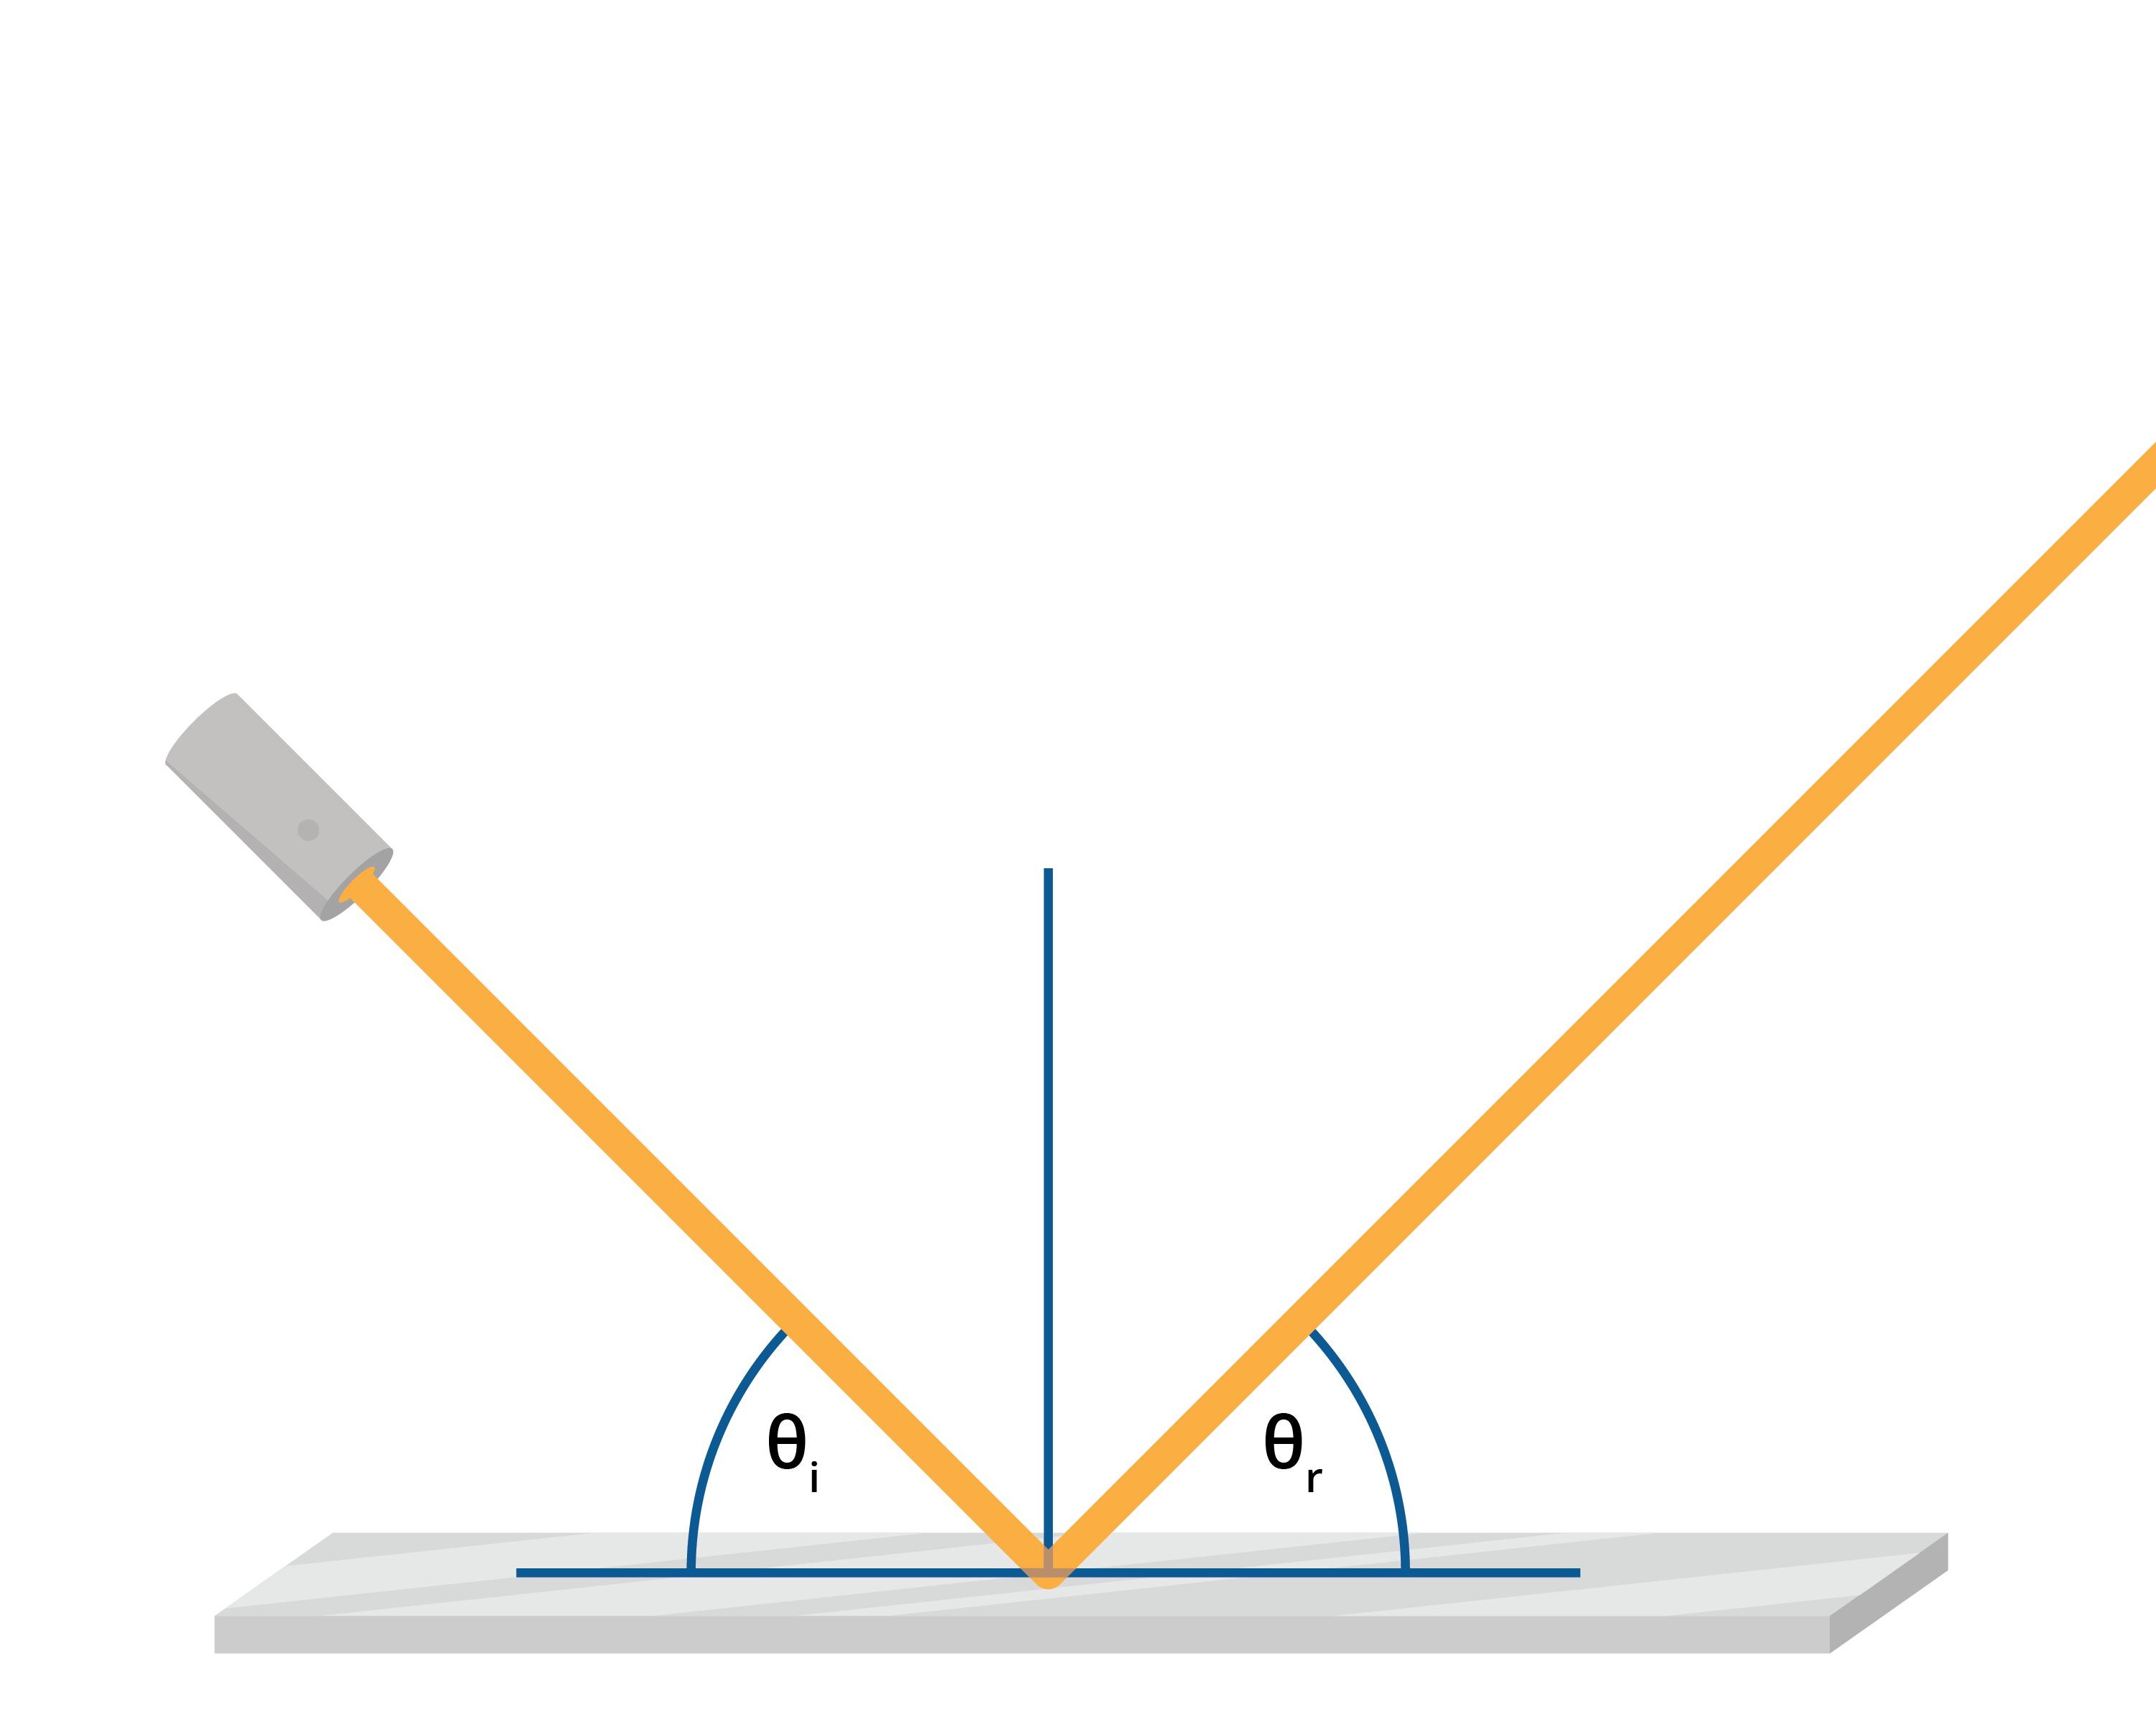
\includegraphics[width=1\textwidth]{reflection.png}

\begin{mdframed}[style=important, frametitle={Law of Reflection}]

The angle of incidence, denoted as $\theta_i$, is equal to
the angle of reflection, denoted as $\theta_r$. This law can be
mathematically expressed as:\index{reflection!law of}

$$\theta_i = \theta_r$$
 
where $\theta_i$ is the angle between the incident light ray and the
normal to the surface, and $\theta_r$ is the angle between the
reflected light ray and the normal.

\begin{tikzpicture}[scale=5]
  \draw [black,thick](-0.7,0)--(0.7,0) node [midway, anchor=north]{Mirror};
  \draw [sdkblue,dashed,->] (0,0) -- (0,0.7) node [anchor=south]{Normal};
  \draw [sdkblue] (0,0.08) -- (0.08, 0.08) -- (0.08, 0);
  \draw [->](-0.5,0.8)--(-0.04,0.05);
  \draw [->](0,0)--(0.5,0.8);
  \draw [sdkblue,<->] (0, 0.3) arc (90:122:0.3)
  node [midway, anchor=south] {$\theta_i$};  
  \draw [sdkblue,<->] (0, 0.3) arc (90:58:0.3)
  node [midway, anchor=south] {$\theta_r$};
\end{tikzpicture}

\end{mdframed}

\begin{Exercise}[title={Law of Reflection}, label=law_of_reflection]

  You are standing 4 meters from a mirror hung on a wall.  The bottom
  of the mirror is the same height as your chin, so you can't see your
  whole body.  You stick a piece of masking tape to your body.

  You walk forward until you are only 3 meters from the mirror, and
  put a piece of masking tape on your body at the new cut-off point.  Is the new
  masking tape higher or lower on your body?
  
\end{Exercise}
\begin{Answer}[ref=law_of_reflection]

 Assuming the mirror is truly vertical and the floor is truly
 horizontal, the new cut off should be exactly the same as the old
 one: It should be below your chin the same amount that your eyes are
 above your chin.

 \textit{Illustration Here}

\end{Answer}

\begin{Exercise}[title={Photons and Color}, label=photon_color]

  There are red photons.

  Are there black photons?

  Are there white photons?

  Are there yellow photons?
  
\end{Exercise}
\begin{Answer}
  
\textit{Are there white photons?}  No. What we call ``white'' is a
blend of photons that are several different colors.

Some people like to say white light is the combination of all visible
colors of photons in equal amounts. That seems oddly specific and unusual.

Maybe it is better to imagine it from the human experience of white
light. In our eyes, we have three different types of color-sensing
cones, which generally correspond to the the red, the green, and the
blue regions of the spectrum.  When all three are excited about equal
amounts, humans experience that as white.  On your computer screen,
for example, what you see as white is just a blend of three colors of
photons: a red, a green, and a blue.

\textit{Are there black photons?}  No. What we call ``black'' is an
absence of photons in the visible range.

\textit{Are there yellow photons?} Yes! There is a region of the color
spectrum that is yellow. It has a wavelength of about 527 nm.  Photons
at this energy level excite both our green-sensitive and red-sensitive
cones.
Your computer monitor does not actually create light with a 527 nm
wavelength. Instead, it creates red light and green light, which our
eyes interpret as yellow.

\end{Answer}

\section{Curved Mirrors}

Flat mirrors are common and useful, but things get more interesting
once you bend the mirrors. In this section, we are going to talk about
a few different kinds of curved mirrors.\index{circle!reflections in}

\subsection{The Reflective Properties of Circles and Spheres}

For example, if you were inside a circular room (a cylinder,
actually), you could imagine standing in the center and pointing a
flash light in any horizontal direction.  The beam of light would
bounce right back to you.

\begin{tikzpicture}[scale=1]
  \coordinate (a) at (0,0);
  \coordinate (b) at ({3 * cos(30)}, {3 * sin(30)});
  \draw [black, thick] (a) circle (3);
  \filldraw [sdkblue] (a) circle (2pt);
  \filldraw [sdkblue] (b) circle (2pt);
  \draw [sdkblue,<->] ({0.2 * cos(30)},{0.2 * sin(30)})--({2.8 * cos(30)},{2.8 * sin(30)});
\end{tikzpicture}

How do you know this?  Because the tangent line is always perpendicular to the radius to the point of tangency:

\begin{tikzpicture}[scale=1.4]
  \coordinate (a) at (0,0);
  \coordinate (b) at ({3 * cos(30)}, {3 * sin(30)});
  \draw [black, thick] (3,0) arc (0:80:3);
  \filldraw [sdkblue] (a) circle (2pt);
  \filldraw [sdkblue] (b) circle (2pt);
  \draw [sdkblue,<->] ({0.2 * cos(30)},{0.2 * sin(30)})--({2.8 * cos(30)},{2.8 * sin(30)});
  \clip (-.1, -.1) rectangle (4,3);
  \draw [dashed] (0,{3 / sin(30)}) -- ({3 / cos(30)},0);
\end{tikzpicture}

You could create a spherical room with mirror walls. You'd
create a platform in the center where you could stand, and if you
pointed your flashlight in any direction, its beam of light would
shine back at you.

\subsection{Ellipses and Ellipsoids}

Intuitively, you know what an ellipse is: it is an oval. But the
ellipse is actually an oval with some special properties.  This is a
good time to talk about those properties.\index{ellipse}

Mathematicians talk about a \newterm{standard} ellipse. A standard ellipse is
centered on the origin $(0,0)$ and its long axis is parallel with the
$x$-axis or the $y$-axis.

\begin{mdframed}[style=important, frametitle={Equation for a Standard Ellipse}]

To be precise, a standard ellipse is the set of points $(x, y)$ that
are solutions to the equation

$$\frac{x^2}{a^2} + \frac{y^2}{b^2} = 1$$


Note that $(a,0), (-a, 0), (0, b), (0,-b)$ are all part of the
set. The complete set looks like this:

\begin{tikzpicture}[scale=2]
  \draw [sdkblue, <->] (-2.5, 0)--(2.5, 0); \draw [sdkblue, <->] (0,
  -1.5)--(0, 1.5); \draw (0,0) ellipse (2 and 1); \filldraw [sdkblue]
  (-2, 0) circle (1pt) node [anchor=east] {$-a$}; \filldraw [sdkblue]
  (2, 0) circle (1pt) node [anchor=west] {$a$}; \filldraw [sdkblue]
  (0, -1) circle (1pt) node [anchor=north] {$-b$}; \filldraw [sdkblue]
  (0, 1) circle (1pt) node [anchor=south] {$b$};
\end{tikzpicture}

The area contained inside this ellipse is given by

$$A = \pi a b$$


\end{mdframed}


We can now talk about two special points: the \newterm{foci}.  Each
focal point is on the long axis of the ellipse.  Let's assume for a
second that $a > b$.  (Everything works the same if $b > a$, but it
gets confusing if we try to deal with both cases simultaneously.)\index{ellipse!focus points}

If $p$ is a point on the ellipse, the distance from $p$ to focal point 1
plus the distance from $p$ to focal point 2 is always $2a$.

\begin{tikzpicture}[scale=2]
  \coordinate (p) at (0.7, 0.93674969975976);
  \coordinate (f1) at (-1.732050807568877, 0);
  \coordinate (f2) at (1.732050807568877, 0);
  \draw [sdkblue, <->] (-2.5, 0)--(2.5, 0);
  \draw [sdkblue, <->] (0, -1.5)--(0, 1.5);
  \draw (0,0) ellipse (2 and 1);
  \filldraw [sdkblue] (-2, 0) circle (1pt) node [anchor=east] {$-a$};
  \filldraw [sdkblue] (2, 0) circle (1pt) node [anchor=west] {$a$};
  \filldraw [sdkblue] (0, -1) circle (1pt) node [anchor=north] {$-b$};
  \filldraw [sdkblue] (0, 1) circle (1pt) node [anchor=south] {$b$};
  \filldraw (p) circle (1pt) node [anchor=south] {$p$};
  \filldraw (f1) circle (1pt) node [anchor=north] {$f_1$};
  \filldraw (f2) circle (1pt) node [anchor=north] {$f_2$};
  \draw [dashed] (f1) -- (p) node [midway, anchor=south] {$d$};
  \draw [dashed] (f2) -- (p) node [midway, anchor=north] {$2a - d$};
\end{tikzpicture}

How do we find the foci? We know they are on the long axis and that
they are symmetrical across the short axis. All we need to know is how
far are they from the short axis.

\begin{mdframed}[style=important, frametitle={Distance from Center to the Foci}]

If you have an ellipse with a long axis that extends $a$ from the center
and a short axis that extends $b$ from the center.  The foci
lie on the long axis and are $c$ from the center.  Where

$$c = \sqrt{a^2 - b^2}$$

\end{mdframed}

\begin{Exercise}[title={Foci of an ellipse}, label=ellipse_foci]
  
You need to draw an ellipse that is 12 cm long and 7 cm wide.  You
have a string, two pushpins, a ruler, and a pencil. Using the ruler,
you draw two perpendicular axes.

You will stick one pin at each focal point.  Each end of the string
will be tied to a push pin. Using the pencil to keep the string taut, you will draw
an ellipse.

\begin{tikzpicture}[scale=.2]
  \coordinate (p) at (-3, 6.77772085586298);
  \coordinate (f1) at (-9.746794344808964, 0);
  \coordinate (f2) at (9.746794344808964, 0);
  \draw [sdkblue, <-] (-14, 0)--(12, 0);
  \draw [sdkblue, <-] (0, -9)--(0, 7);
  \draw (0,0) ellipse (12 and 7);
  \filldraw [sdkblue] (-12, 0) circle (4pt);
  \filldraw [sdkblue] (12, 0) circle (4pt) node [anchor=west] {12 cm};
  \filldraw [sdkblue] (0, -7) circle (4pt);
  \filldraw [sdkblue] (0, 7) circle (4pt) node [anchor=south] {7 cm};
  \filldraw (p) circle (4pt) ;
  \filldraw (f1) circle (4pt);
  \filldraw (f2) circle (4pt);
  \draw [dashed] (f1) -- (p);
  \draw [dashed] (f2) -- (p);
\end{tikzpicture}

How far from the short axis are the pushpins placed?

How long is the string between them?

\end{Exercise}
\begin{Answer}[ref=ellipse_foci]

  The length of the string is easy: $2 \times 12 = 24$ cm.

  The distance from the center to the focal point is $\sqrt{12^2 - 7^2} approx 6.78$ cm.

  \begin{tikzpicture}[scale=.2]
  \coordinate (p) at (-3, 6.77772085586298);
  \coordinate (f1) at (-9.746794344808964, 0);
  \coordinate (f2) at (9.746794344808964, 0);
  \draw [sdkblue, <-] (-14, 0)--(12, 0);
  \draw [sdkblue, <-] (0, -9)--(0, 7);
  \draw (0,0) ellipse (12 and 7);
  \filldraw [sdkblue] (-12, 0) circle (4pt);
  \filldraw [sdkblue] (12, 0) circle (4pt) node [anchor=west] {12 cm};
  \filldraw [sdkblue] (0, -7) circle (4pt);
  \filldraw [sdkblue] (0, 7) circle (4pt) node [anchor=south] {7 cm};
  \filldraw (p) circle (4pt) ;
  \filldraw (f1) circle (4pt);
  \filldraw (f2) circle (4pt);
  \draw [dashed] (f1) -- (p) node [midway, anchor=south] {$d$};
  \draw [dashed] (f2) -- (p) node [midway, anchor=south] {$24 - d$};
  \draw (6,0) node [anchor=north] {6.78 cm};
\end{tikzpicture}

\end{Answer}

\subsubsection{The Reflective Property of Ellipses}

Here is something else that is wonderful about an ellipse: Pick any
point $p$ on the ellipse. Draw a line from $p$ to each focal point.
Draw the line tangent to the ellipse at $p$.  Fact: The angle between
the tangent and the line to focal point 1 is equal to the angle between the
tangent and the line to focal point 2.

\begin{tikzpicture}[scale=2]
  \coordinate (p) at (0.7, 0.93674969975976);
  \coordinate (f1) at (-1.732050807568877, 0);
  \coordinate (f2) at (1.732050807568877, 0);
  \clip (-2.5, -.4) rectangle (5.5,2);
  \draw [sdkblue] (-2.1, 0)--(2.1, 0);
  \draw [sdkblue] (0, -1.1)--(0, 1.1);
  \draw (0,0) ellipse (2 and 1);
  \filldraw (p) circle (1pt) node [anchor=south] {$p$};
  \filldraw (f1) circle (1pt) node [anchor=north] {$f_1$};
  \filldraw (f2) circle (1pt) node [anchor=north] {$f_2$};
  \draw [sdkblue] (f1) -- (p);
  \draw [sdkblue] (f2) -- (p);
  \coordinate (t1) at (-0.2829937278, 1.120388832);
  \coordinate (t2) at (1.682993728, 0.7531105671); 
  \draw [dashed, thick]  (t1)--(t2);
  \draw [sdkblue, <->] (t1) arc (169.4181988:201.0651201:1)
     node [midway, anchor=east] {$\theta$};
  \draw [sdkblue, <->] (t2) arc (-10.5818012:-42.22872252:1)
     node [midway, anchor=east] {$\theta$};
\end{tikzpicture}

This is known as ``The Reflective Property of Ellipses.''

Imagine you and your friend Fred are at an ellipse-shaped skating rink and
edge of the rink are mirrored.  You sit at one focal point and your friend
sits at the other, if you point a flashlight at the mirror (in any
direction!) the beam will bounce off the wall and head directly for
Fred.

If Fred ducks out of the way, the beam will bounce again and
head back to you.

\begin{tikzpicture}[scale=4]
  \coordinate (p) at (0.7, 0.93674969975976);
  \coordinate (p2) at (1.95763,-0.204758);
  \coordinate (f1) at (-1.732050807568877, 0);
  \coordinate (f2) at (1.732050807568877, 0);
  \draw (0,0) ellipse (2 and 1);
  \filldraw [sdkblue] (p) circle (0.5pt);
  \filldraw [sdkblue] (p2) circle (0.5pt);
  \filldraw (f1) circle (1pt) node [anchor=north] {You};
  \filldraw (f2) circle (1pt) node [anchor=north] {Fred};
  \draw [sdkblue, ->] (f1) -- (p);
  \draw [sdkblue, ->] (p) -- (p2);
  \draw [sdkblue, ->] (p2) -- (f1);
  \coordinate (b1) at (0.6081804337,0.4452528358);
  \coordinate (b2) at (1.219613217,0.1039995564);
  \draw [dashed] (p)--(b1);
  \draw [dashed] (p2)--(b2);
  \coordinate (t1) at (0.1102037633, 1.046933179);
  \coordinate (t2) at (1.289796237, 0.8265662202); 
  \draw [dashed, thick]  (t1)--(t2);
  \draw [dashed, thick] (1.764656527,-0.6660184891) -- (2.150603473,0.2565024891);
  \draw [sdkblue, <->] (b1) arc (-100.5818012:-42.22872252:0.5)
     node [midway, anchor=south] {$\theta_1$};
  \draw [sdkblue, <->] (b1) arc (-100.5818012:-158.9348799:0.5)
     node [midway, anchor=south] {$\theta_1$};
  \draw [sdkblue, <->] (b2) arc (157.2974596:137.7712775:0.8)
     node [midway, anchor=west] {$\theta_2$};
  \draw [sdkblue, <->] (b2) arc (157.2974596:176.8236417:0.8)
     node [midway, anchor=west] {$\theta_2$};
\end{tikzpicture}

This will work for sound too.  If you whisper on the focal point, Fred
(at the other focal point) will hear you surprisingly well because all
the soundwaves that hit the wall will bounce (just like the light)
straight at Fred.

\subsection{Elliptical Orbits}

One more fun fact about ellipses: We often imagine the planets
traveling in circular orbits with the sun at the center -- they
actually travel in elliptical orbits, with the sun as one of the focal
points.\index{orbit!elliptical}

The earth is closest to the sun around January 3rd: 147 million km.

The earth is farthest from the sun around July 3rd: 152 million km.

(Note that these dates are not the same as the solstices: The southern
hemisphere is tilted the most toward the sun around December 21 and
tilted most away around June 21.)

\subsection{Ellipsoids}

Just as we can pull the ideas of a circle into three dimensions to
make a sphere, we can extend the ideas of the ellipse into three
dimensions to talk about ellipsoids.  Ellipsoids are like blimps.\index{ellipsoid}

The standard ellipsoids are centered at the origin and aligned with the three axes.

\begin{mdframed}[style=important, frametitle={Equation for a Standard Ellipsoid}]

To be precise, a standard ellipse is the set of points $(x, y, z)$ that
satify the equation

$$\frac{x^2}{a^2} + \frac{y^2}{b^2} + \frac{z^2}{c^2}= 1$$


Note that $(a,0,0), (0, b,0), (0,0,c)$ are all part of the
set. The complete set looks like this:

\begin{tikzpicture}[scale=2.0]
  \begin{axis}[
    view={35}{15},
    unit vector ratio=1 1 1,
    ticks = none,
    axis lines=middle,
    ymin=-4.0,
    ymax=4.0,
    xmin=-3.5,
    xmax=3.5,
    zmin=-1.5,
    zmax=1.5,
    x axis line style=<->,
    y axis line style=<->,
    z axis line style=<->,
    clip=false
  ]
    \addplot3[samples y=0,domain=0:360,smooth,dashed,sdkblue]({3*cos(x)}, {2*sin(x)},0);
    \addplot3[surf,shader=interp,domain=0:360,y domain=0:180, opacity=0.5,
    colormap={blackwhite}{color=(black) color=(black!30)}] ({3 * sin(y) * cos(x)},
    {2*sin(y)* sin(x)},{1*cos(y)});
    \addplot3[samples y=0,domain=0:360,smooth,sdkblue](0, {2*sin(x)},{1*cos(x)});
    \addplot3[samples y=0,domain=0:180,smooth]({3* cos(x)}, 0,{1*sin(x)});
  \end{axis}
  \end{tikzpicture}

  The volume bounded by this ellipsoid is

    $$V = \frac{4}{3} \pi a b c$$


\end{mdframed}

Of course, $a$, $b$, and $c$ can be any positive number, but in the
real world we find ourselves working a lot with ellipsoids where two
of the numbers are the same.

\subsubsection{Oblate Spheroid}

If two axes have the same length and one is shorter, you get something
that looks like a sphere compressed in one direction -- like a
pumpkin.  These are called \newterm{oblate spheroids}.\index{oblate spheroid}

The earth is actually an oblate spheroid: the axis that goes through
the north and south pole is shorter than the axes that pass through
the equator.  How much shorter? Just a little: The equator is 6,378 km
from the center of the earth. The north pole is 21 km closer.\index{earth!shape of}

\subsubsection{Prolate Spheroid}

If two axes have the same length and one is longer, you get something
that looks like a sphere stretched in one direction -- like a rugby
ball. It is called a \newterm{prolate spheroid}.\index{prolate spheroid}

Like an ellipse, prolate spheroids have two focal points.

\begin{mdframed}[style=important, frametitle={Focal Points of a Prolate Spheroid}]

  If the long axis has a radial length of $a$ and the two shorter axes
  have radial length $b$, then the focal points are on the long axis.  The distance from the center to the focal point is given by

  $$c = \sqrt{a^2 - b^2}$$

  For any point $p$ on the prolate spheroid, the sum of the distances
  from $p$ to the focus points will always be $2a$.

  It has the reflective property: A photon shot in any any direction
  from one focal point will bounce off the wall and head directly at the other.
  
\end{mdframed}

\begin{Exercise}[title={Volume of Ruby Ball}, label=rugby_ball]

  Some jokesters once thought it would be fun to make something that looked like a rugby ball, but made out of lead.

  A rugby ball is about 30 cm long and has a circumference of 60 cm at
  its midpoint. A cubic centimeter of lead has a mass of 11.34 grams.

  How much would a solid (not hollow) lead ruby ball weigh?

\end{Exercise}
\begin{Answer}[ref=rugby_ball]

  We need the distance from the center out to each of the three axes.  We know that $a = \left(\frac{1}{2} \right) 30 = 15$ cm.

  We can calculate the $b$ and $c$ (which are equal) using the circumference given: $2b\pi = 60$, so $c = b \approx 9.55$ cm.

  The volume, then is
  
  $$V = \frac{4}{3} \pi (15)(9.55)(9.55) \approx 5,730 \text{ cubic centimeters }$$ 

  The mass would be $5,730 \times 11.34 = 64,973$ grams or about 65 kg.
\end{Answer}
  
\subsection{Parabolas and Parabolic Reflectors}

You are familiar with quadratic functions:

$$y = a x^2 + b x + c$$

If $a$ is not zero, the graph of a quadratic is a curved line called a
\newterm{parabola}.  The first parabola that most mathematicians think of is the graph of $y = x^2$:

\begin{tikzpicture}
    \draw[sdkblue,<->] (-2.0, 0) -- (2.0, 0) node[right] {$x$};
    \draw[sdkblue,<->] (0, -1) -- (0, 5) node[above] {$y$};
    \draw[domain=-1.9:1.9,samples=300,variable=\x,<->]  plot (\x,{\x*\x});
    \draw (1.1, 1) node [anchor=west] {$y = x^2$};
\end{tikzpicture}

Every parabola has a \newterm{focus} and a \newterm{directix}.  The
focus is a point on the parabola's axis of symmetry.  The directrix is
a line perpendicular to the axis of symmetry.  Every point on the
parabola is equal distance from the focus and the directrix.

For the graph of $y = x^2$, the focus is the point $(0, \frac{1}{4})$.  The directrix is the line $y = -\frac{1}{4}$:

\begin{tikzpicture}
  \coordinate (f) at (0, 1/4);
  \coordinate (p) at (1.25,1.5625);
  \coordinate (pd) at (1.25,-1/4);
  \draw[sdkblue,<->] (-2.5, 0) -- (2.5, 0) node[right] {$x$};
  \draw[sdkblue,<->] (0, -1) -- (0, 5) node[above] {$y$};
  \draw[domain=-2.2:2.2,samples=300,variable=\x,<->]  plot (\x,{\x*\x});
  \draw (2, 4) node [anchor=west] {$y = x^2$};
  \filldraw (f) circle (2pt);
  \filldraw  (p) circle (1pt);
  \filldraw  (pd) circle (1pt);
  \draw [dashed, thin] (f) -- (p) -- (pd);
  \draw [dashed, <->, thick] (-2.5, -1/4) -- (2.5, -1/4);
  \draw (1.25, -0.05) -- (1.45,-0.05) -- (1.45, -1/4);
\end{tikzpicture}

For example, the point $(1,1)$ is on this parabola. It is 5/4 from the
directorix. How far is it from the focus?  1 horizontally and 3/4 vertically.

$$\sqrt{1^2 + \left( \frac{3}{4} \right)^2} = \frac{5}{4}$$

Thus, we have confirmed that $(1,1)$ is equal distances from the focus
and the directrix.

When we think about a parabola and its properties, we usually rotate
and translate it to be symmetric around the $y$-axis, flip it so that
it is low in the middle and rising on both sides, and push it up or
down until the low point is is on the $x$-axis.

Then, they can all be written:

$$y = \frac{a}{4} x^2$$

where $a > 0$. If $a$ is small, the parabola opens wider.

\begin{tikzpicture}
  \coordinate (f) at (0, 1/4);
  \draw[sdkblue,<->,thin] (-2.5, 0) -- (2.5, 0) node[right] {$x$};
  \draw[sdkblue,->,thin] (0, 0) -- (0, 2.5) node[above] {$y$};
  \draw[sdkblue, domain=-1.5:1.5, samples=300, variable=\x, <->,thick]  plot (\x,{\x*\x})
  node [anchor=south] {$a = 4$};
  \draw[domain=-2.2:2.2,samples=300,variable=\x,<->,thick]  plot (\x,{0.125*\x*\x})
  node [anchor=west] {$a = 0.5$};
\end{tikzpicture}

Then the focus is at $(0, \frac{1}{a})$ and the directorix is the line $y = -\frac{1}{a}$.

\begin{tikzpicture}
  \coordinate (f1) at (0, 1/4);
  \coordinate (p1) at (1, 1);
  \coordinate (p1d) at (1, -0.25);
  \coordinate (f2) at (0, 2);
  \coordinate (p2) at (-1.5, 0.28125);
  \coordinate (p2d) at (-1.5, -2);
  \draw[sdkblue,<->,thin] (-2.5, 0) -- (2.5, 0);
  \draw[sdkblue,<->,thin] (0, -2.5) -- (0, 2.5);
  \draw[sdkblue, domain=-1.5:1.5, samples=300, variable=\x, <->, thick]  plot (\x,{\x*\x})
  node [anchor=south] {$a = 4$};
  \filldraw [sdkblue] (f1) circle (2pt);
  \filldraw [sdkblue] (p1) circle (1pt);
  \filldraw [sdkblue] (p1d) circle (1pt);
  \draw [sdkblue,dashed, thick] (-2.5, -0.25)--(2.5, -0.25) node [anchor=west]{$y=-\frac{1}{4}$};
  \draw [sdkblue,thin,dashed] (f1) -- (p1) -- (p1d);
  \draw[domain=-2.2:2.2,samples=300,variable=\x,<->, thick]  plot (\x,{0.125*\x*\x})
  node [anchor=west] {$a = 0.5$};
  \filldraw  (f2) circle (2pt) node [anchor=west] {$(0,2)$};
  \filldraw  (p2) circle (1pt);
  \filldraw  (p2d) circle (1pt);
  \draw [dashed, thick] (-2.5, -2)--(2.5, -2) node [anchor=west]{$y=-2$};;
  \draw [thin,dashed] (f2) -- (p2) -- (p2d);
\end{tikzpicture}

\subsubsection{Reflective Property of a Parabola}

Assume you have a parabola-shaped mirror, a beam of light shot from
the focus, will bounce of the mirror in the direction of axis of
symmetry:

\begin{tikzpicture}
  \coordinate (f2) at (0, 2);
  \coordinate (p1) at (1, 0.125);
  \coordinate (p1d) at (1, 3);
  \coordinate (p2) at (-1.5, 0.28125);
  \coordinate (p2d) at (-1.5, 3);
  \coordinate (p3) at (2, 0.5);
  \coordinate (p3d) at (2, 3);
  \coordinate (p4) at (-0.5, 0.03125);
  \coordinate (p4d) at (-0.5, 3);
  \draw[sdkblue,thick] (0, 0) -- (0, 2.0);
  \draw[domain=-2.2:2.2,samples=300,variable=\x,<->, thick]  plot (\x,{0.125*\x*\x});
  \filldraw  (f2) circle (2pt);
  \filldraw  (p1) circle (1pt);
  \draw [thin,dashed,->] (f2) -- (p1) -- (p1d);
  \filldraw  (p2) circle (1pt);
  \draw [thin,dashed,->] (f2) -- (p2) -- (p2d);
  \filldraw  (p3) circle (1pt);
  \draw [thin,dashed,->] (f2) -- (p3) -- (p3d);
  \filldraw  (p4) circle (1pt);
  \draw [thin,dashed,->] (f2) -- (p4) -- (p4d);
\end{tikzpicture}

This is why your flashlight has a parabolic mirror: the lightbulb is
at the focus so any photons that hit the mirror are redirected
straight forward.

(Note that in the real world, we use parabolic dishes: a rotated around its axis of
symmetry.)

The reflection works exactly the same in reverse: There are solar
cookers that are big parabolic mirrors.  They let you put a pot on the
focus point.  You move the dish until its axis of symmetry is pointed
at the sun.

You will also see a lot of antennas have parabolic dishes. Note that
photons that come in parallel to the axis of symmetry are redirected
to a single point -- where the receiver is.

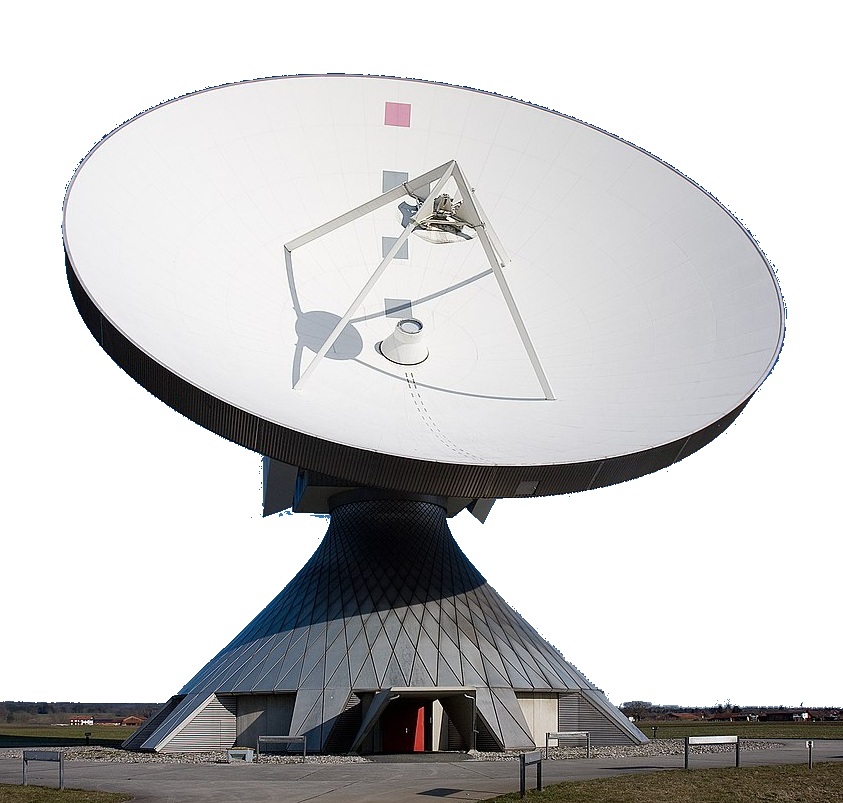
\includegraphics[width=0.7\linewidth]{dish.png}



Sometimes in a science museum, you will see two parabolic dishes far
apart and pointed at each other.  One person speaks with their mouth
at the focus of one.  The other person listens with their ear at the
focus of the other. Even though you are very far apart, it sounds like
they are really, really close.

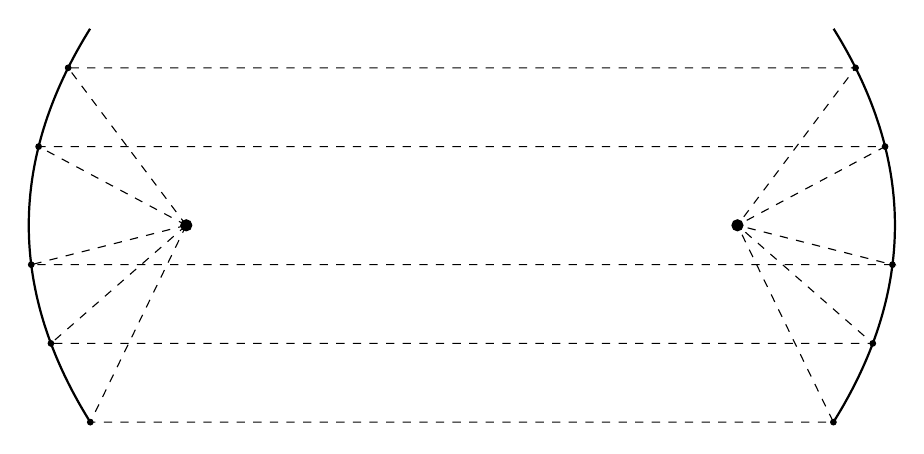
\begin{tikzpicture}
  \coordinate (f1) at (9, 0);
  \coordinate (f2) at (2, 0);
  \coordinate (p1) at (0.125, 1);
  \coordinate (p1d) at (10.875,1);
  \coordinate (p2) at (0.28125,-1.5);
  \coordinate (p2d) at (10.71875, -1.5);
  \coordinate (p3) at (0.5,2);
  \coordinate (p3d) at (10.5, 2);
  \coordinate (p4) at (0.03125, -0.5);
  \coordinate (p4d) at (10.96875, -0.5);
  \coordinate (p5) at (0.78125, -2.5);
  \coordinate (p5d) at (10.21875, -2.5);
  \draw[domain=-2.5:2.5,samples=300,variable=\x, thick]  plot ({0.125*\x*\x},\x);
  \draw[domain=-2.5:2.5,samples=300,variable=\x, thick]  plot ({11 - 0.125*\x*\x},\x);
  \filldraw  (f1) circle (2pt);
  \filldraw  (f2) circle (2pt);
  \filldraw  (p1) circle (1pt);
  \filldraw  (p1d) circle (1pt);
  \draw [thin,dashed] (f2) -- (p1) -- (p1d) -- (f1);
  \filldraw  (p2) circle (1pt);
  \filldraw  (p2d) circle (1pt);
  \draw [thin,dashed] (f2) -- (p2) -- (p2d) -- (f1);
  \filldraw  (p3) circle (1pt);
  \filldraw  (p3d) circle (1pt);
  \draw [thin,dashed] (f2) -- (p3) -- (p3d)--(f1);
  \filldraw  (p4) circle (1pt);
  \filldraw  (p4d) circle (1pt);
  \draw [thin,dashed] (f2) -- (p4) -- (p4d) -- (f1);
  \filldraw  (p5) circle (1pt);
  \filldraw  (p5d) circle (1pt);
  \draw [thin,dashed] (f2) -- (p5) -- (p5d) -- (f1);
\end{tikzpicture}

This is because the speaker's parabolic wall focuses the sound energy
in a nice beam the size of the wall pointed straight at the listener's
parabolic wall.  The listener's wall focuses the energy of that beam
at the listener's ear.


\graphicspath{{../../Chapters/refraction/en_US}}
\chapter{Refraction}


Refraction of light is the phenomenon where light changes its direction when it passes from one medium to another. The change in direction is due to a change in the speed of light as it moves from one medium to another. 

This phenomenon is explained by Snell's law, which states:

\begin{equation}
n_1 \cdot \sin(\theta_1) = n_2 \cdot \sin(\theta_2)
\end{equation}

where:
\begin{itemize}
\item $n_1$ and $n_2$ are the indices of refraction for the first and second media, respectively. The index of refraction is the ratio of the speed of light in a vacuum to the speed of light in the medium. It is a dimensionless quantity.
\item $\theta_1$ and $\theta_2$ are the angles of incidence and refraction, respectively. These angles are measured from the normal (perpendicular line) to the surface at the point where light hits the boundary.
\end{itemize}

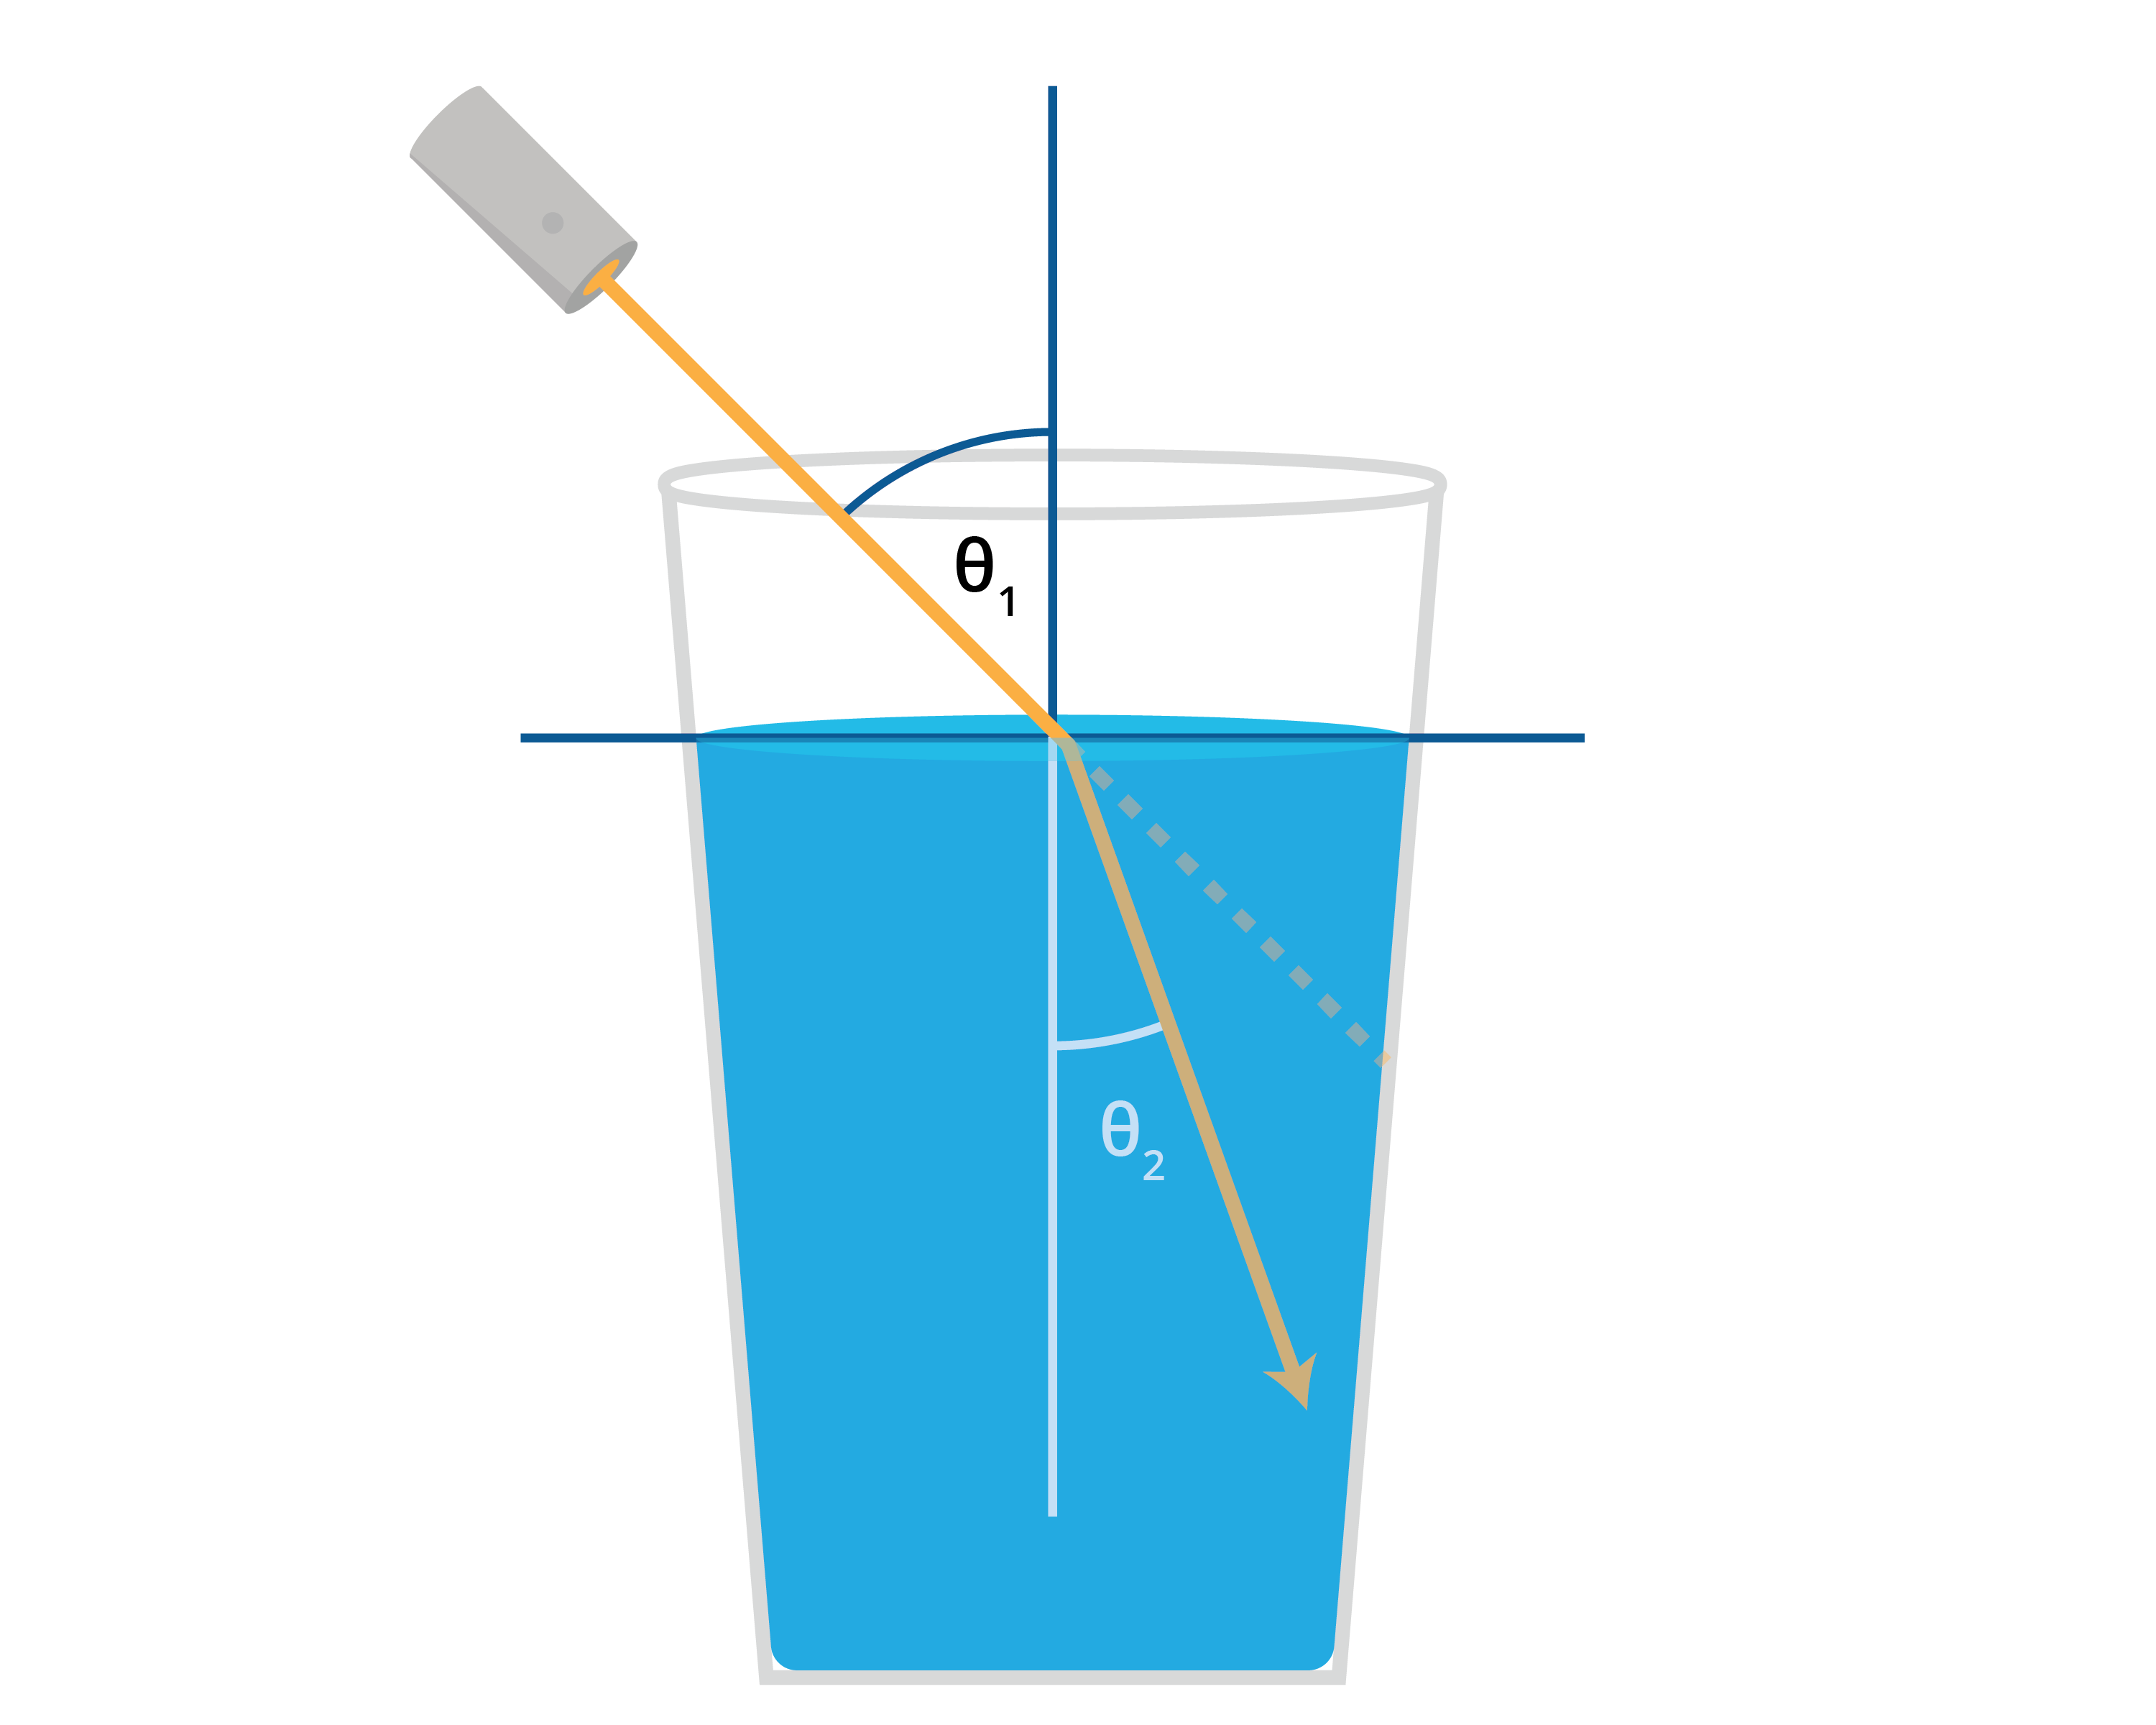
\includegraphics[width=.75\textwidth]{refraction.png}

The angle of incidence ($\theta_1$) is the angle between the incident ray and the normal to the interface at the point of incidence. Similarly, the angle of refraction ($\theta_2$) is the angle between the refracted ray and the normal.

When light travels from a medium with a lower refractive index to a medium with a higher refractive index, it bends towards the normal. Conversely, when light travels from a medium with a higher refractive index to one with a lower refractive index, it bends away from the normal.


\graphicspath{{../../Chapters/lens/en_US}}
\chapter{Lenses}

Lenses are optical devices with perfect or approximate axial symmetry
that transmit and refract light, converging or diverging the
beam. There are two main types of lenses, distinguished by their shape
and the way they refract light:\index{lenses}

\begin{itemize}
    \item \textbf{Converging (or Convex) Lenses:} These are thicker at
      the center than at the edges. When parallel light rays enter a
      convex lens, they converge to a point called the focal
      point. Examples of converging lenses include magnifying glasses
      and camera lenses.

      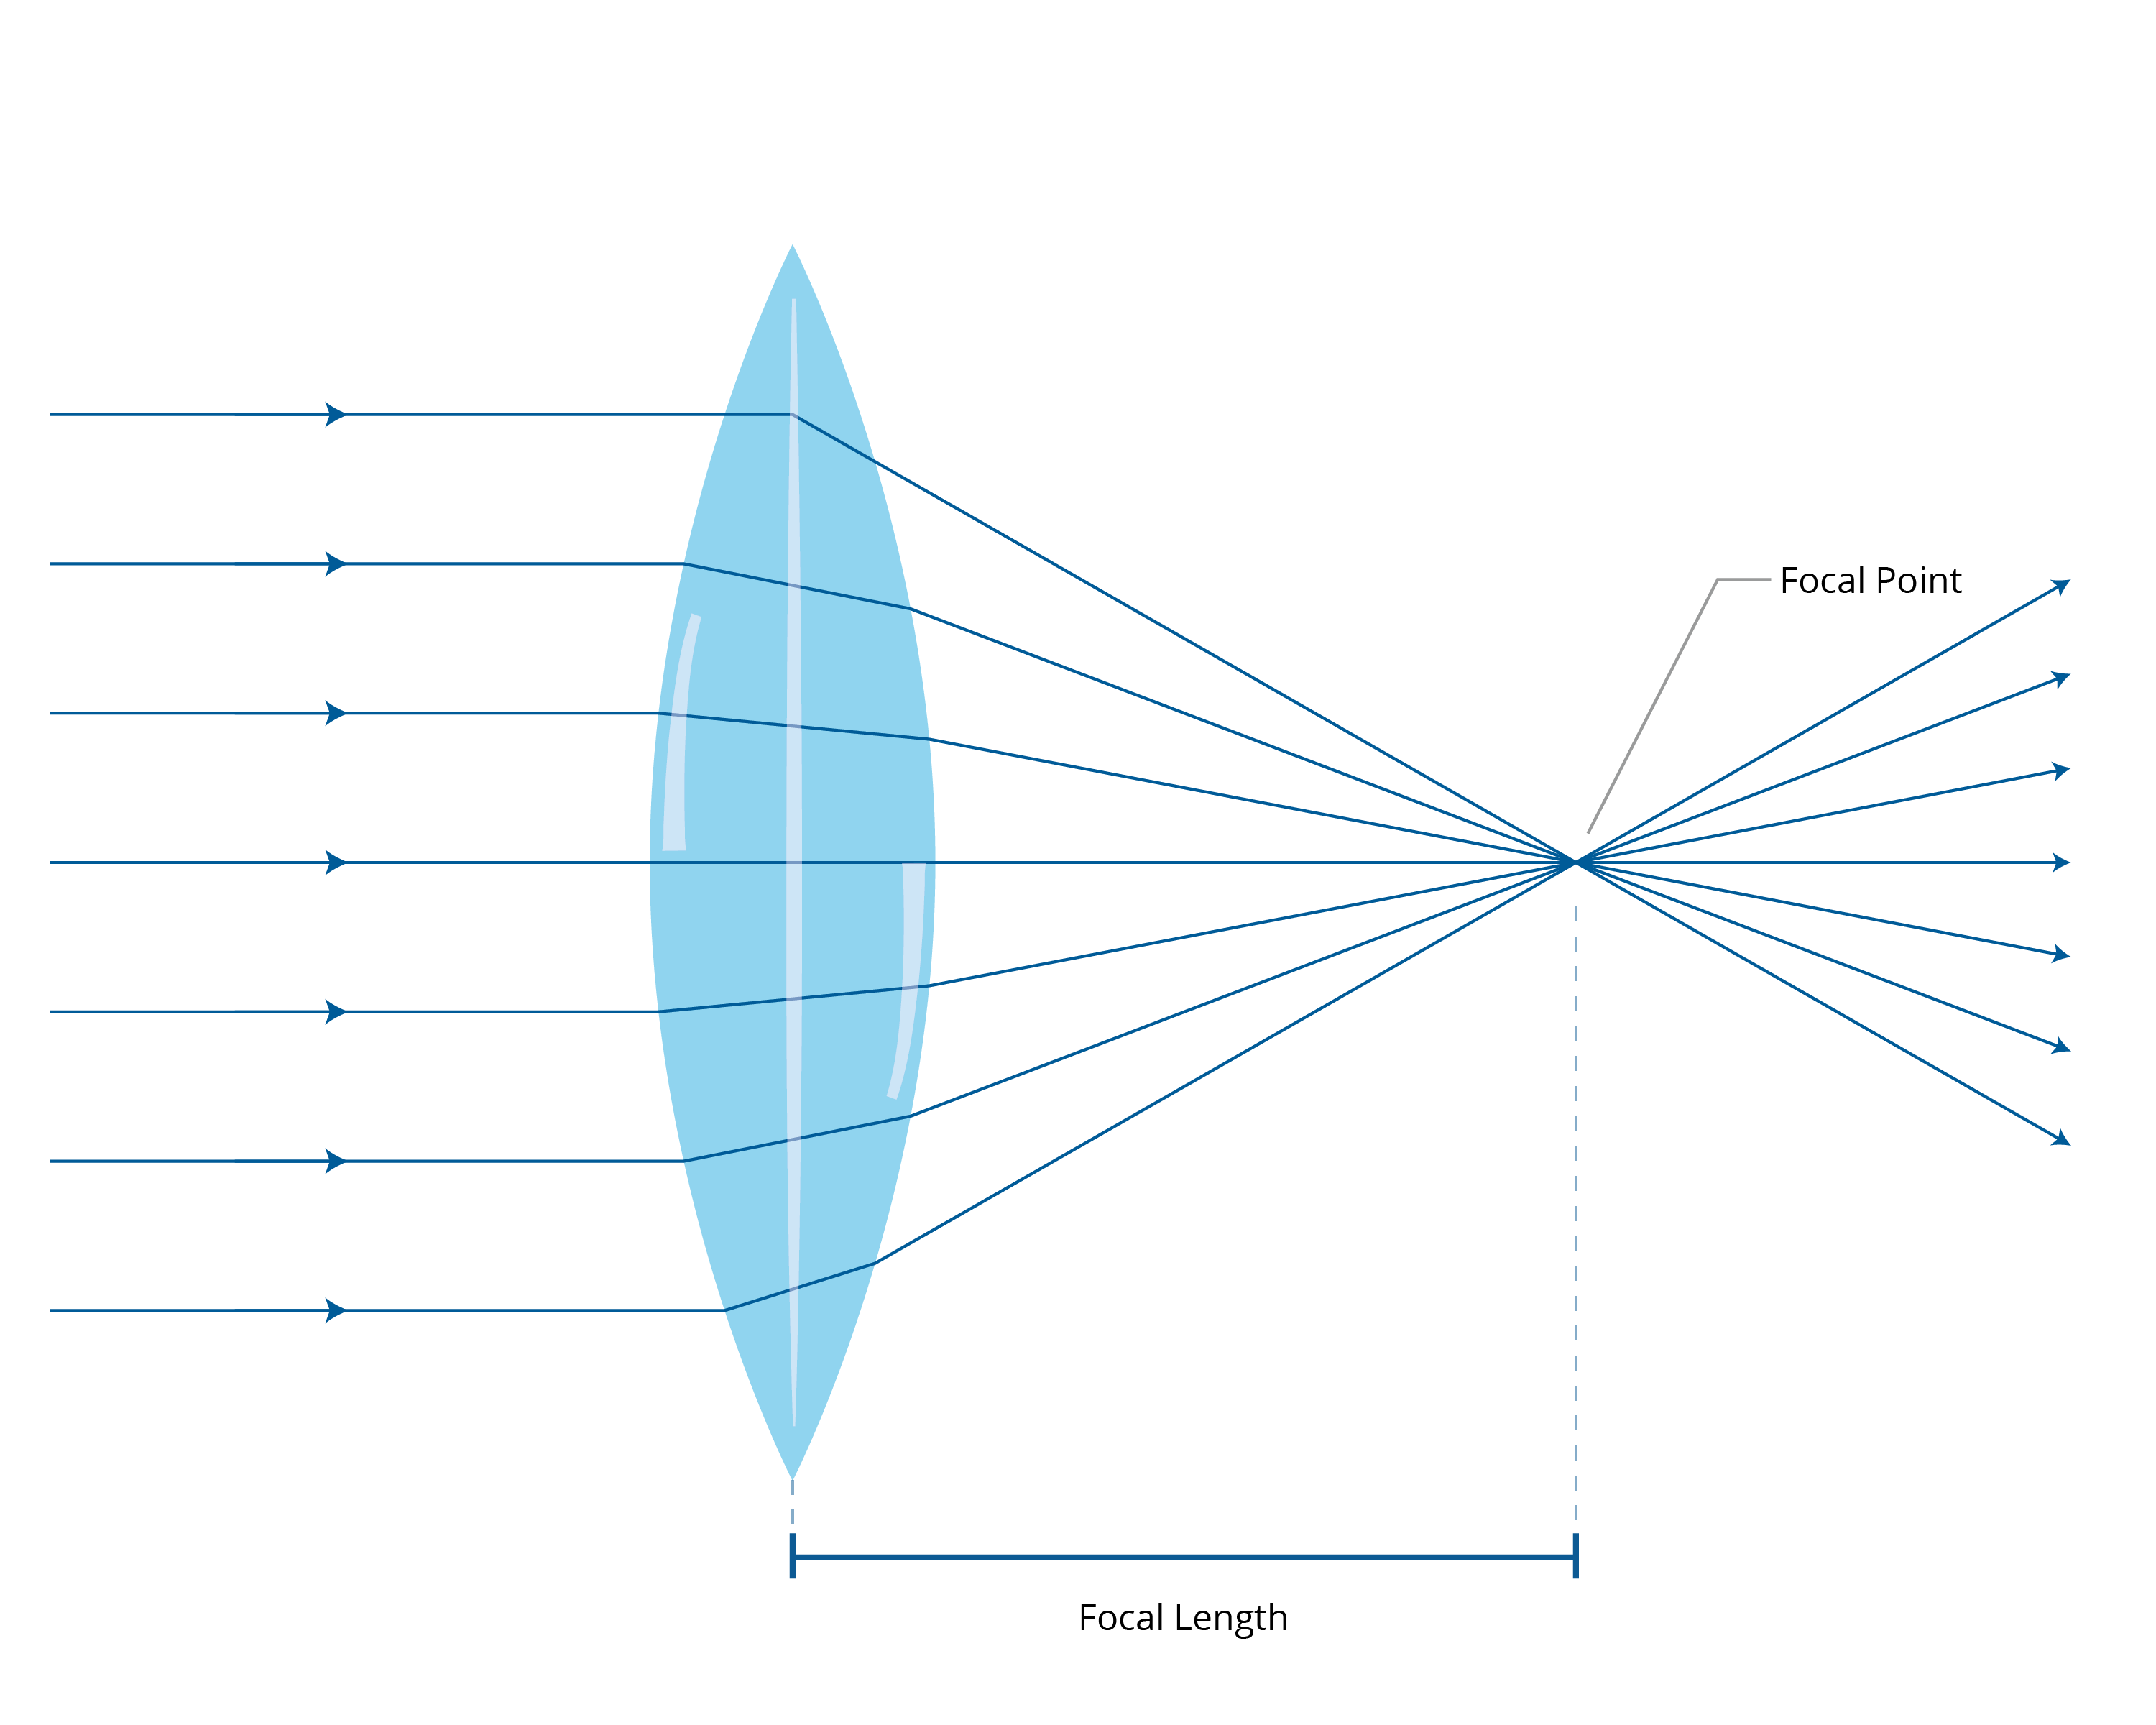
\includegraphics[width=0.5\textwidth]{convex.png}

    \item \textbf{Diverging (or Concave) Lenses:} These are thinner at
      the center than at the edges. When parallel light rays enter a
      concave lens, they diverge or spread out. These lenses are often
      used in glasses to correct nearsightedness.
      
      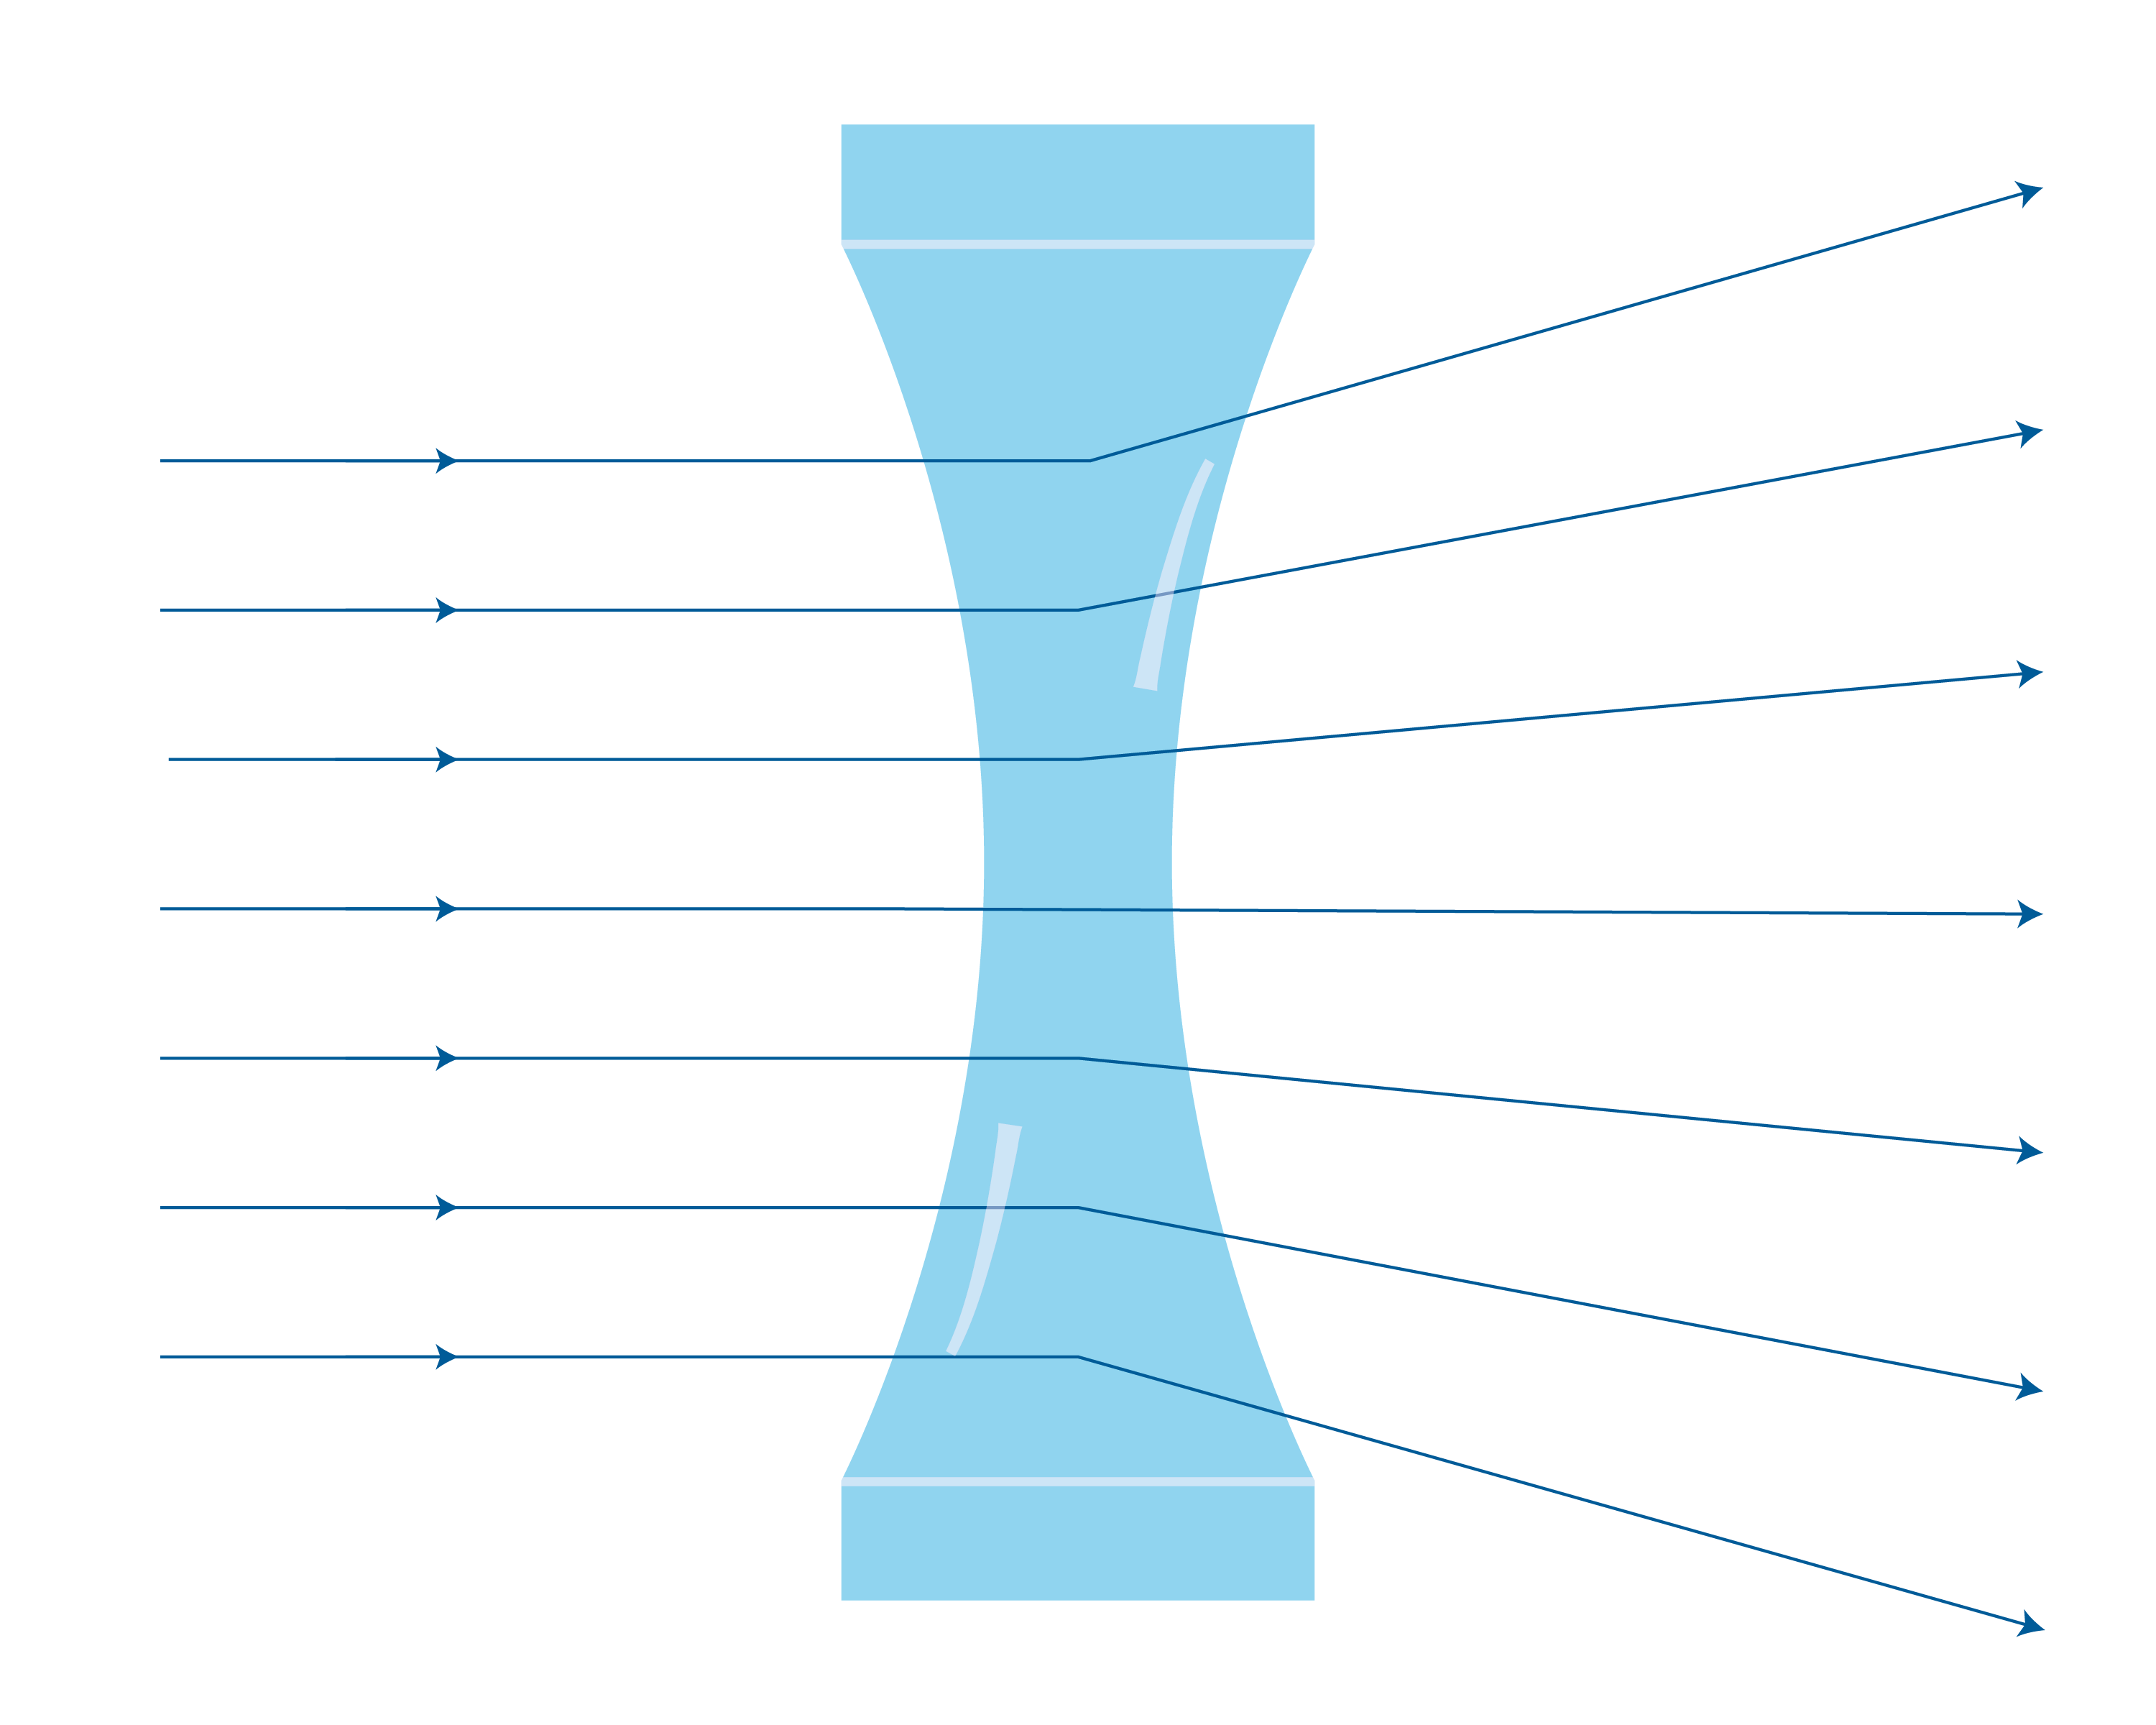
\includegraphics[width=0.5\textwidth]{concave.png}

\end{itemize}

\section{Focal Length}

The focal length of a lens is the distance between the center of the
lens and the focal point. It is determined by the lens shape and the
refractive index of the lens material. For a converging lens, the
focal length is positive, and for a diverging lens, the focal length
is negative.\index{focal length}

\section{Refractive Index}

The refractive index of a material is a measure of how much the speed
of light is reduced inside the material. The refractive index $n$ of a
material is given by the ratio of the speed of light in a vacuum $c$
to the speed of light $v$ in the material:\index{refractive index}

\[
n = \frac{c}{v}
\]

The refractive index affects how much a light ray changes direction,
or refracts, when entering the material at an angle. A higher
refractive index indicates that light travels slower in that medium
and the light ray will bend more towards the normal.

Lenses work by refracting light at their two surfaces. By choosing the
right lens shape and material, lenses can be designed to bring light
to a focus, spread it out, or perform more complex transformations.

\graphicspath{{../../Chapters/py_images/en_US}}
\chapter{Images in Python}

An image is usually represented as a three-dimensional array of 8-bit
integers. NumPy arrays are the most commonly used library for this
sort of data structure.

If you have an RGB image that is 480 pixels tall and 640 pixels wide,
you will need a $480 \times 640 \times 3$ NumPy array.

There is a separate library (imageio) that:
\begin{itemize}
\item Reads an image file (like JPEG files) and creates a NumPy array.
\item Writes a NumPy array to a file in standard image formats
\end{itemize}

Let's create a simply python program that creates a file containing an
all-black image that is 640 pixels wide and 480 pixels tall. Create a
file called \filename{create\_image.py}:

\begin{Verbatim}
import NumPy as np
import imageio
import sys

# Check command-line arguments
if len(sys.argv) < 2:
    print(f"Usage {sys.argv[0]} <outfile>")
    sys.exit(1)

# Constants
IMAGE_WIDTH = 640
IMAGE_HEIGHT = 480

# Create an array of zeros
image = np.zeros((IMAGE_HEIGHT, IMAGE_WIDTH, 3), dtype=np.uint8)

# Write the array to the file
imageio.imwrite(sys.argv[1], image)
\end{Verbatim}

To run this, you will need to supply the name of the file you are
trying to create. The extension (like .png or .jpeg) will tell imageio
what format you want written. Run it now:

\begin{Verbatim}
python3 create_image.py blackness.png
\end{Verbatim}

Open the image to confirm that it is 640 pixels wide, 480 pixels tall, and completely black.

\section{Adding color}

Now, let's walk through through the image, pixel-by-pixel, adding some
red. We will gradually increase the red from 0 on the left to 255 on
the right.

\begin{Verbatim}[commandchars=\\\{\}]
import NumPy as np
import imageio
import sys

# Check command-line arguments
if len(sys.argv) < 2:
    print(f"Usage {sys.argv[0]} <outfile>")
    sys.exit(1)

# Constants
IMAGE_WIDTH = 640
IMAGE_HEIGHT = 480

# Create an array of zeros
image = np.zeros((IMAGE_HEIGHT, IMAGE_WIDTH, 3), dtype=np.uint8)

\textbf{for col in range(IMAGE_WIDTH):}

    \textbf{# Red goes from 0 to 255 (left to right)}
    \textbf{r = int(col * 255.0 / IMAGE_WIDTH)}

    \textbf{# Update all the pixels in that column}
    \textbf{for row in range(IMAGE_HEIGHT):}
        \textbf{# Set the red pixel}
        \textbf{image[row, col, 0] = r}

# Write the array to the file
imageio.imwrite(sys.argv[1], image)
\end{Verbatim}

When you run the function to create a new image, it will be a fade
from black to red as you move from left to right:

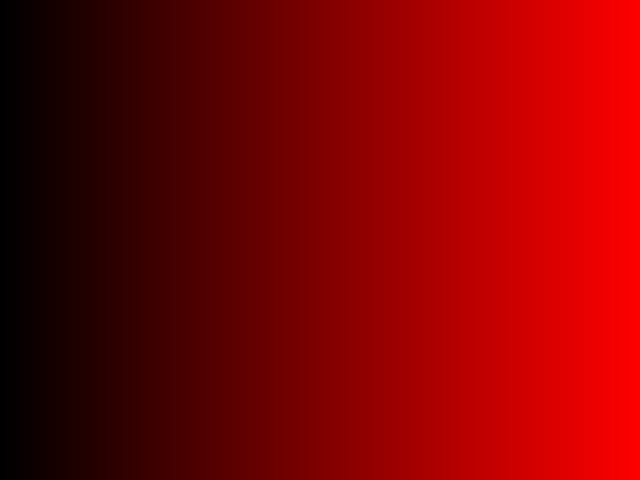
\includegraphics[width=0.4\linewidth]{red.png}

Now, inside the inner loop, update the blue channel so that it goes
from zero at the top to 255 at the bottom:

\begin{Verbatim}[commandchars=\\\{\}]
    # Update all the pixels in that column
    for row in range(IMAGE_HEIGHT):

        # Update the red channel
        image[row,col,0] = r
        
        \textbf{# Blue goes from 0 to 255 (top to bottom)}
        \textbf{b = int(row * 255.0 / IMAGE_HEIGHT)}
        \textbf{image[row,col,2] = b}

imageio.imwrite(sys.argv[1], image)
\end{Verbatim}

When you run the program again, you will see the color fades from
black to blue as you go down the left side. As you go down the right
side, the color fades from red to magenta.

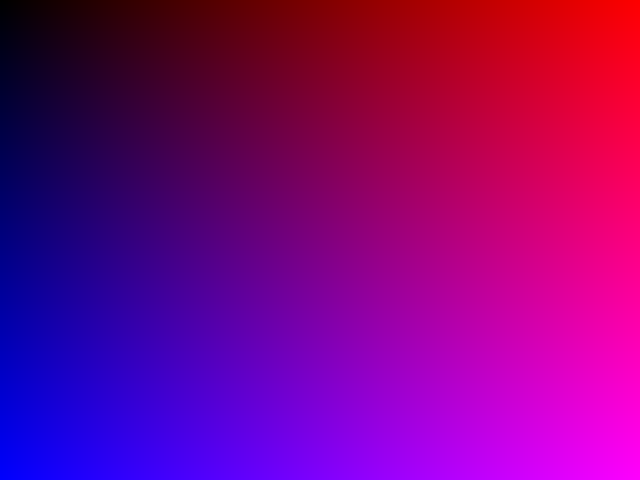
\includegraphics[width=0.4\linewidth]{rb.png}

Notice that red and blue with no green looks magenta to your eye.

Now let's add some stripes of green:

\begin{Verbatim}[commandchars=\\\{\}]
import NumPy as np
import imageio
import sys

# Check command line arguments
if len(sys.argv) < 2:
    print(f"Usage {sys.argv[0]} <outfile>")
    sys.exit(1)

# Constants
IMAGE_WIDTH = 640
IMAGE_HEIGHT = 480
\textbf{STRIPE_WIDTH = 40}
\textbf{pattern_width = STRIPE_WIDTH * 2}

# Create an image of all zeros
image = np.zeros((IMAGE_HEIGHT, IMAGE_WIDTH, 3), dtype=np.uint8)

# Step from left to right
for col in range(IMAGE_WIDTH):

    # Red goes from 0 to 255 (left to right)
    r = int(col * 255.0 / IMAGE_WIDTH)

    \textbf{# Should I add green to this column?}
    \textbf{should_green = col % pattern_width > STRIPE_WIDTH}

    # Update all the pixels in that column
    for row in range(IMAGE_HEIGHT):

        # Update the red channel
        image[row,col,0] = r

        \textbf{# Should I add green to this pixel?}
        \textbf{if should_green:}
            \textbf{image[row,col,1] = 255}

        # Blue goes from 0 to 255 (top to bottom)
        b = int(row * 255.0 / IMAGE_HEIGHT)
        image[row,col,2] = b

imageio.imwrite(sys.argv[1], image)
\end{Verbatim}

When you run this version, you will see the previous image in half the
stripes.  In the other half, you will see that green fades to cyan
down the left side and yellow fades to white down the right side.

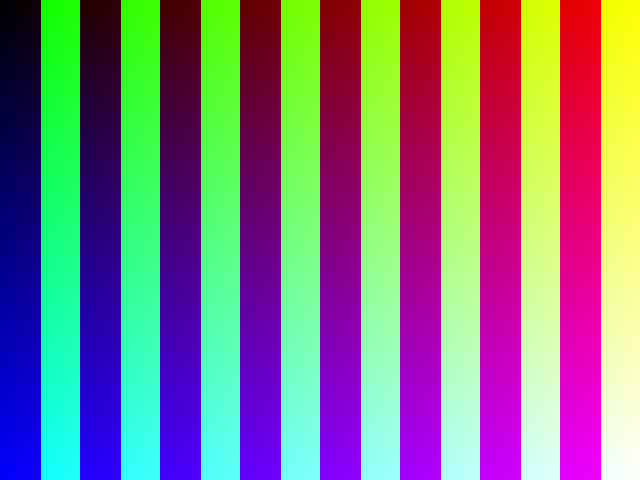
\includegraphics[width=0.4\linewidth]{rgb.png}

\section{Using an existing image}

imageio can also be used to read in any common image file
format. Let's read in an image and save each of the red, green, and blue
channels out as its own image.

Create a new file called \filename{separate\_image.py}:

\begin{Verbatim}
import imageio
import sys
import os

# Check command line arguments
if len(sys.argv) < 2:
    print(f"Usage {sys.argv[0]} <infile>")
    sys.exit(1)

# Read the image
path = sys.argv[1]
image = imageio.imread(path)

# What is the filename?
filename = os.path.basename(path)

# What is the shape of the array?
original_shape = image.shape

# Log it
print(f"Shape of {filename}:{original_shape}")

# Names of the colors for the filenames
colors = ['red','green','blue']

# Step through each of the colors
for i in range(3):

    # Create a new image
    newimage = np.zeros(original_shape, dtype=np.uint8)

    # Copy one channel
    newimage[:,:,i] = image[:,:,i]

    # Save to a file
    new_filename = f"{colors[i]}_{filename}"
    print(f"Writing {new_filename}")
    imageio.imwrite(new_filename, newimage)
\end{Verbatim}

Now you can run the program with any common RGB image type:

\begin{Verbatim}
python3 separate_image.py dog.jpg
\end{Verbatim}

This will create three images: \filename{red\_dog.jpg},
\filename{green\_dog.jpg}, and \filename{blue\_dog.jpg}.

%%%%%%%%%%%%%%%%%%%%%%%%%%%%%%%%%
%% Bookfooter.tex by Aaron Hillegass
%% Nov 8, 2020

\appendix

\chapter{Answers to Exercises}
\shipoutAnswer

\bibliography{references}

\printindex

\end{document}